\documentclass[a4paper]{elsarticle}
\usepackage{graphicx,amssymb,color,url,amscd,stmaryrd,supertabular,amsmath,tikz,cancel}
\usetikzlibrary{shapes,snakes,arrows,automata,calc}

\def\qed{\relax\ifmmode\hskip2em \blacksquare\else\unskip\nobreak\hfill\hskip1em \fi}
\def\exqed{\relax\ifmmode\hskip2em \diamond\else\unskip\nobreak\hfill\hskip1em \fi}



\newcommand\Zed{\mathbb{Z}}
\newcommand\Nen{\mathbb{N}}
\newcommand{\ZZ}{\mathbb{Z}}
\newcommand{\NN}{\mathbb{N}}
\newcommand\PPP{\mathcal{P}}
\newcommand\card[1]{\left|{#1}\right|}

\newcommand{\ACA}{\mathcal{A}}
\newcommand{\ACB}{\mathcal{B}}
\newcommand{\ACC}{\mathcal{C}}
\newcommand{\ACD}{\mathcal{D}}
\newcommand{\ACX}{\mathcal{X}}
\newcommand{\ACU}{\mathcal{U}}
\newcommand{\locA}{f_{\ACA}}
\newcommand{\locB}{f_{\ACB}}
\newcommand{\locC}{f_{\ACC}}
\newcommand\glob[1]{G_{#1}}
\newcommand\local[1]{f_{#1}}
\newcommand{\globA}{G_{\ACA}}
\newcommand{\globB}{G_{\ACB}}
\newcommand{\globC}{G_{\ACC}}
\newcommand{\globX}{G_{\ACX}}
\newcommand\alphabe[1]{S_{#1}}
\newcommand{\alphA}{\alphabe{\ACA}}
\newcommand{\alphB}{\alphabe{\ACB}}
\newcommand{\alphC}{\alphabe{\ACC}}
\newcommand{\radA}{r_{\ACA}}
\newcommand{\radB}{r_{\ACB}}


\newcommand\sfop[1]{\operatorname{\hbox{\usefont{T1}{cmss}{m}{n}#1}}}
\newcommand\sfbop[1]{\operatorname{\hbox{\usefont{T1}{cmss}{bx}{n}#1}}}
\newcommand\utrans{\sfop{Trans}}
\newcommand\opapp{\sfbop{apply}}
\newcommand\opdiv{\sfbop{divide}}
\newcommand\opcom{\sfbop{combine}}
\newcommand\tPmCS{\sfbop{\~{P}CS}}


\newcommand{\unif}{\overline}
\newcommand\sac{\sqsubseteq}
\newcommand{\sacby}[1]{\sqsubseteq_{#1}}
\newcommand{\fac}{\trianglelefteq}
\newcommand{\facby}[1]{\trianglelefteq_{#1}}
\newcommand{\facsac}{\fac\!\sac}
\newcommand\bulk[2]{{#1}^{\left\langle{#2}\right\rangle}}
\newcommand{\simu}{\preccurlyeq}
\newcommand{\sacsimu}{\simu_i}
\newcommand{\facsimu}{\simu_s}
\newcommand{\facsacsimu}{\simu_m}
\newcommand{\sime}{\sim}
\newcommand{\sacsime}{\sime_i}
\newcommand{\facsime}{\sime_s}
\newcommand{\facsacsime}{\sime_m}
\newcommand{\simc}[1]{\left[{#1}\right]}
\newcommand{\sacsimc}[1]{\left[{#1}\right]_i}
\newcommand{\facsimc}[1]{\left[{#1}\right]_s}
\newcommand{\facsacsimc}[1]{\left[{#1}\right]_m}
\newcommand{\isom}{\equiv}
\newcommand{\locrelset}{\mathcal{R}}
\newcommand\blocss[1]{\Sigma_{#1}}

\newcommand\grporder{\leqslant_\square}
\newcommand\grp[2]{{#1}^{[#2]}}
\newcommand\grpclass[1]{\left[{#1}\right]_{\Box}}
\newcommand\bloc[1]{\Box^{#1}}
\newcommand\debloc[1]{\Box^{-#1}}

\newcommand\MTM{\mathcal{M}}
\newcommand\statM{S_\MTM}
\newcommand\rubM{Q_\MTM}
\newcommand\transM{\phi_\MTM}
\newcommand\mtape{\chi_Q}
\newcommand\mhead{\chi_S}
\newcommand\nohead{\epsilon}

\newcommand\dist{d}


\newcommand\sing{\bot}
\newcommand\univ{\mathfrak{U}}
\newcommand\zee[1]{\mathcal{Z}_{#1}}
\newcommand\shi[2]{\sigma_{{#1},{#2}}}
\newcommand\carashi[1]{\chi\left({#1}\right)}
\newcommand\metro{\mathcal{M}}
\newcommand{\limprod}[1]{{\ACA}_\infty}
\newcommand\blc[1]{\texttt{B}_{#1}}
\newcommand\flagseq[1]{u_{#1}}

\newcommand\equi{\mathcal{T}_1}
\newcommand\equipt{\mathcal{T}_2}
\newcommand\sensi{\mathcal{T}_3}
\newcommand\expansi{\mathcal{T}_4}
\newcommand\fami{\mathfrak{F}}
\newcommand\cod{\phi}

\newcommand\deci[1]{\textsc{#1}}
\newcommand\aperdettiling{\deci{Aper-Det-Tiling}}
\newcommand\nilper{\deci{Nil-Per}}

\newtheorem{defn}{Definition}[section]
\newtheorem{thm}{Theorem}[section]
\newtheorem{lm}{Lemma}[section]
\newtheorem{ex}{Example}[section]
\newproof{pf}{Proof}
\newtheorem{openpb}{Open Problem}
\newtheorem{cor}{Corollary}[section]



\newcommand\TODO[2]{{\color{red}\par\noindent\textbf{#1.} #2}}
\newcommand\inTODO[1]{{\color{red}#1}}
\newcommand{\BIB}[1]{{\color{green!30!blue}\scriptsize\textbf{[BIB: #1]}}}
\newcommand{\ic}[1]{
  \begin{flushright}
    \fbox{\begin{minipage}{.6\linewidth}
      \textit{#1}
    \end{minipage}}
  \end{flushright}}




\begin{document}

\begin{frontmatter}
  \title{Bulking II: Classifications of Cellular Automata\tnoteref{phd}}
  \tnotetext[phd]{The results presented here first appeared to a great extent in French in the PhD theses of Ollinger~\cite{Ollinger:2002:PhD} and Theyssier~\cite{Theyssier:2005:PhD}}
  \author[lip]{M. Delorme}
  \author[lip]{J. Mazoyer}
  \author[lif]{N. Ollinger}
  \author[lama]{G. Theyssier\corref{cora}} 
  \cortext[cora]{Corresponding author
    (\url{Guillaume.Theyssier@univ-savoie.fr})}

  \address[lip]{LIP, ENS Lyon, CNRS, 46 all\'ee d'Italie,
    69\hspace{0.2em}007 Lyon, France} \address[lif]{LIF, Aix-Marseille
    Universit\'e, CNRS, 39 rue Joliot-Curie, 13\hspace{0.2em}013
    Marseille, \rlap{France}} \address[lama]{LAMA, Universit\'e de
    Savoie, CNRS, 73\hspace{0.2em}376 Le Bourget-du-Lac Cedex, France}

\begin{abstract}
  This paper is the second part of a series of two papers dealing with
  bulking: a way to define quasi-order on cellular automata by
  comparing space-time diagrams up to rescaling.  In the present
  paper, we introduce three notions of simulation between cellular
  automata and study the quasi-order structures induced by these
  simulation relations on the whole set of cellular automata. Various
  aspects of these quasi-orders are considered (induced equivalence
  relations, maximum elements, induced orders, etc) providing several
  formal tools allowing to classify cellular automata.
\end{abstract}

\begin{keyword}
cellular automata\sep bulking\sep grouping\sep classification
\end{keyword}
\end{frontmatter}

\section{Introduction}
\label{sec:intro}

In the first paper \cite{bulking1}, we have developped a general theory of
bulking aimed at defining quasi-orders on cellular automata based on the idea of
space-time rescaling. The present paper focuses on three instances of such
quasi-orders and uses them as classification tools over the set of
one-dimensional cellular automata.

Classifying does not make sense without additional assumptions (some
criteria of classification). If in Wolframs
papers~\cite{Wolfram:1984:CTCA} these criteria were implicit and
informal, several classifications with explicit and formal criteria
have been since
proposed~\cite{Gilman:1987:CLA,Cattaneo:1999:TDD,Kurka97}. Usually,
the criteria are those of dynamical systems and consist in a finite
list of qualitative behaviors. Our approach here is different: we
don't define any \textit{a priori} list of behaviors. Instead, we
consider a simulation relation (a quasi-order) which tells when some
cellular automaton is able to reproduce the behavior of another. The
criterion of classification is then the definition of the
quasi-order. Our central thesis is that, when it comes to apprehend
the great variety of behaviors in cellular automata, the language of
orders (equivalence classes, chains, ideals, maximal elements,
distance to the bottom, etc) is more adapted than a finite list of
monadic predicates (of the form ``having property P'' for some P).

In this paper, we introduce three quasi-orders. They are all defined
according to the same scheme developped in the companion paper
\cite{bulking1}: some local comparison relation up to spatio-temporal
rescaling. They only differ in the local comparison they use, which
are based on the two following basic notions:
\begin{itemize}
\item the \emph{injection} of a small system () \emph{into} a larger one (),
\item the \emph{projection} of a large system () \emph{onto} a smaller one ().
\end{itemize}

The three quasi-orders can be defined informally as follows:
\begin{itemize}
\item an \emph{injective} simulation of  by , denoted by , is an injection of some rescaling of  into some
  rescaling of ;
\item a \emph{surjective} simulation of  by , denoted by , is the projection of some rescaling of  onto some
  rescaling of ;
\item a \emph{mixed} simulation of  by , denoted by , is the injection into some rescaling of  of some
   that projects onto some rescaling of .
\end{itemize}

In the context of cellular automata, the two notions of local
comparison above (injection and projection) translate into the
following.  The first notion is the \emph{subautomaton} relation (
obtained from  by forgetting some states) and the second one is the
\emph{quotient} relation ( obtained from  by identifying some
sates). 

The subautomaton relation was already introduced in \cite{bulking1}
and its importance in cellular automata is illustrated by theorems 4
and 5 of that paper. 

The quotient relation can be seen as a particular case of the notion
of factor in dynamical systems theory and symbolic dynamics
(homomorphism between shift-commuting continuous global maps,
see~\cite{LindMarcus}). More intuitively, the quotient relation is a
means to extract coarse-grained information () from a complex
system () (see \cite{physcoarsegrained}). For instance, the
metaphor of particles moving in a stable background used in the
literature of cellular automata\cite{Boccara} follows this idea: some
information (e.g. the phase of the background) is hidden by
identification of states. However, our definition of quotient requires
that both  (the original system) and  (the one obtained after
identification of some states) are cellular
automata. 



We study these orders with several points of view and aim at
understanding their structure as well as showing that they suitably
capture many classical properties or phenomena of cellular automata.

For instance, concerning the phenomenon of universality, we show that
orders  and  have a maximum, that classes
of CA having Turing-universality can be obtained by simulating (in a
way closed to Smith~III~\cite{Smith:1971:SCU}) a universal Turing
machine, and that such a class is not necessarily at the top of the
order.

As another example, we show that many global properties of cellular
automata as dynamical systems (reversibility, sensitivity,
expansivity, etc) or cellular automata as computational devices
(ability to simulate a Turing head, or to propagate some signal) characterize
an ideal or a filter in our orders.





\paragraph{Overview of the paper} Section~\ref{sec:def} introduces
three different comparison relations which are three different
instances of the bulking theory developed in the companion paper
\cite{bulking1}.  Section~\ref{sec:co} sets the definitions of these
three notions of simulations and establishes some of their basic
properties. Section~\ref{sec:bot} studies the 'bottom' of each of the
three quasi-orders induced on CA, \textit{i.e.} CA or classes of CA of
least complexity. Section~\ref{sec:sp} focuses on the order structure
with respect to various classical properties of CA, and from a
computability point of view. Then section~\ref{sec:top} explores the
set of CA at the 'top' of these quasi-orders: universal CA. Once
again, the point of view is both structural and computational.
Finally, section~\ref{sec:io} is devoted to the construction of
noticeable induced orders (like infinite chains), and the study of how
simple families of CA spread over these quasi-orders.


\subsection{Definitions}
\label{sec:def}

In this paper, we adopt the setting of one-dimensional cellular
automata with a canonical neighborhood (connected and centered).  A
cellular automaton (CA) is a triple  where:
\begin{itemize}
\item  is the (finite) \emph{state set},
\item  is the neighborhood \emph{radius},
\item  is the \emph{local transition function}.
\end{itemize}

A coloring of the lattice  with states from 
(\textit{i.e.}  an element of ) is called a
\emph{configuration}.  To  we associate a global function
 acting on configurations by synchronous and uniform
application of the local transition function.  Formally,  is defined by:
 for all .  Several
CA can share the same global function although there are syntactically
different (different radii and local functions). However we are mainly
interested in global functions and will sometimes define CA through
their global function without specifying particular syntactical
representations. In addition, the Curtis-Heldund-Lyndon theorem
\cite{Hedlund:1969} allows us to freely compose global CA functions to
construct new CA without manipulating explicitly the underlying
syntactical representation.

When dealing with several CA simultaneously, we use index notation to
denote their respective state sets, radii and local functions. For
instance, to  we associate ,  and .

This paper will make an intensive use of  transforms defined
in section 4.2 of \cite{bulking1}, but restricted to dimension 1. With
this restriction, a  transform  has the form
 where  and  are
positive integers,  is a (possibly negative) integer and  is
either  or .

For any CA , we denote by  or more
explicitly  the application of  to
, which is, according to notations of \cite{bulking1}, a CA of
state set  and global rule:

To simplify notation we will use a shortcut for purely temporal
transforms: for any CA  we denote by  the CA
. Finally, as another special case, we denote
by  the grouped instance of  of parameter : it
corresponds to the transform 
(see~\cite{bulking1} for a detailed exposition of grouping).

\section{Canonical orders}
\label{sec:co}

In this section we introduce the three bulking quasi-orders that are
studied all along the paper. They are obtained by applying the bulking
axiomatics developed in the companion paper \cite{bulking1} to three
'canonical' relations between local rules of CA.

Those thee 'canonical' relations are in turn based on two classical
notions of morphism between local transition rules of CA:
sub-automaton and quotient-automaton. As shown below, the three
relations we consider are exactly the reflexive and transitive
relations that can be defined by compositions of one or more such
morphisms.


\subsection{From Three Local Relations to Three Bulking Quasi-Orders}
\label{sec:canondef}

A \emph{sub-automaton} is a restriction of a CA to a stable
sub-alphabet. A \emph{quotient} is a projection of a CA onto a smaller
alphabet and compatible with the local transition rule\footnote{A
  quotient is a particular kind of \emph{factor}, a classical notion
  in dynamical systems theory and symbolic dynamics \cite{kurkabook}}.
Both define a kind of morphism between cellular automata:

\begin{itemize}
\item  is a \emph{sub-automaton} of , denoted
  , if there is an injective map
   such that
  , where
   denotes the
  uniform extension of . We often write 
  to make the map  explicit.
    
\item  is a \emph{quotient} of , denoted ,
  if there is a surjective (onto) map  from  to 
  such that , where
   denotes the uniform
  extension of . We also write  to make the map
   explicit.
\end{itemize}

Relations  and  are quasi-orders (reflexive and
transitive) and it is straightforward to check that their induced
equivalence relation is the relation of isomorphism between cellular
automata (equality up to state renaming) denoted by .

It is also straightforward to check that  and  are
incomparable (none of them is implied by the other one). It is thus
interesting to consider compositions of them. The composition of two
relations  and  is the relation  defined by

We denote by  the set of relations obtained by (finite)
composition of  and . Any relation of  is a
priori interesting, but the following theorem justifies that we
restrict to ,  and the composition  only.  In
the sequel  is denoted by  and, as for  and
, we use the infix notation ().

\begin{thm}
  \label{thm:locrel}
  \par\noindent
  \begin{enumerate}
  \item any relation  is included in 
    (\textit{i.e., } implies ) ;
  \item the transitive relations of  are exactly: ,
     and .
  \end{enumerate}
\end{thm}
\begin{pf}
  We first prove that if  then
  , which is sufficient to prove assertion 1 by
  transitivity of  and of .  So consider , 
  and  such that  and
  . Then consider . We
  have  because
  \newcommand\cmtinproof[1]{\ \text{(#1)}}
  
The CA 
  is thus well-defined and by definition we have
  . Moreover, we have  because  is
  well-defined and onto, and because
  
  since  and
   over
  .  Hence
   and assertion 1 is proven.

  Given assertion 1 we have . To prove assertion 2, it is thus sufficient to prove
  that  is not transitive.  To do this, consider
   with  prime, , and let
   be five distinct elements of
  . Then consider , the CA with state set ,
  radius  and local rule  defined by:
    depends only on two variables. Suppose now
  that there is some AC  with at least two states such that
  . We will show that  must be one-to-one.
  Suppose for the sake of contradiction that there are distinct
  elements  and  in  such that . Then,
  because  for any , we have
   and more generally  for all . So, supposing
  without loss of generality , let . We deduce from
  above that  for all  and, by
  elementary group theory, that  is constant equal to 
  (because  is prime and ).  This is in contradiction with
  the fact that  has image  which has at least two
  elements. So  is one-to-one and  is isomorphic to
  . Now consider , the identity CA over state set
  . Since  possesses  quiescent states and
   has no quiescent state (straightforward from the definition
  of  above), we have .  With the
  discussion above, we can conclude that
  .

  However, we have  because the states
   induce a sub-automaton  of 
  which verifies  where  is defined by 
  et . Assertion 2 follows since the relation  is
  included in the composition of the relation  with
  itself. \qed
\end{pf}

Like  (already considered in \cite{bulking1}),  and
 are quasi-orders on CA and therefore constitute natural
candidates for the  relation of bulking axiomatics (definition
8 of \cite{bulking1}).

Inspired by definition 14 of \cite{bulking1}, we now define 3 bulking
quasi-orders using  transforms.  

\begin{defn}
   simulates  \emph{injectively}, denoted
  , if there exist two  transforms
   and  such that
  .
\end{defn}

We will occasionally use the notion of simulation by grouping
introduced in \cite{Mazoyer:1999:IOC} and discussed in
\cite{bulking1}: we denote by  the fact that
there are  and  such that
. This is a special case of the
injective simulation above.

\begin{defn}
   simulates  \emph{surjectively}, denoted
  , if there exist two  transforms
   and  such that
  .
\end{defn}

\begin{defn}
   simulates  in a mixed way, denoted
  , if there exist two  transforms
   and  such that
  
\end{defn}

For each notion of simulation above, we say that the simulation is
\emph{strong} if the transformation  applied to the simulated
CA is trivial:  so that
.

\begin{thm}
  ,  and
   are quasi-orders.
\end{thm}
\begin{pf}
  We show that  and  correspond exactly to
  models of bulking developped in \cite{bulking1}: the proof of
  theorem 15 of \cite{bulking1} contains the case of injective
  simulation. The case of  follows immediately (axiom
   is straightforward and axiom  is verified because
   contains ). For , the proof of each axiom
  is similar except for axiom .



  With or without axiom , theorem 10 of \cite{bulking1} can be
  applied in each case and show the present theorem.\qed
\end{pf}


\begin{lm}
  \label{lem:mapa}
  Let  be any relation among ,  and . Then the following
  propositions are equivalent:
  \begin{itemize}
  \item there exist two  transforms  and  such that
    ,
  \item there exist a  transform  and an integer  such that
    ,
  \item there exist a  transform  and an integer  such that
    ,
  \end{itemize}
\end{lm}
\newcommand\trsfo[1]{\left\langle #1, 0\right\rangle}
\begin{pf}
  We use the property of compatibility of relation  with respect
  to geometrical transforms (axiom  of \cite{bulking1}).  The lemma follows
  from the following property: for any transform , there exist a
  transform  and an integer  such that
  
  If ,  can be chosen as the composition of
  ,  and .\qed
\end{pf}


In the sequel, if  denotes a simulation quasi-order we denote
by  the induced equivalence relation and by  the
equivalence class of  with respect to . For instance, to
 we associate the notations  and
 with the following meanings:

 We use similar notations for  and
.



Before entering into details concerning various aspects of the three
simulation relations defined above, we can already make a clear (yet
informal) distinction between  and  on one hand,
and  on the other hand. For the two former, the simulation
takes place on a subset of configurations and nothing can be said
\textit{a priori} about the behavior of the simulator outside this
subset of configurations. For , however, the simulation
occurs on any configuration and the simulator's behavior on any
configuration is in some way affected by the
simulation. Section~\ref{sec:idfi} give several illustrations of this
difference.

\subsection{First Properties}
\label{sec:firstprop}

We now establish a set of basic general facts about ,
 and  while next sections of the paper focus on
particular aspects.

\begin{thm}
  \label{thm:bfacts}
  Let  be any CA and  be any relation among ,
   and . Then it holds:
  \begin{enumerate}
  \item there is some  having a quiescent state,
  \item there is some  with radius ,
  \item  where  is the CA with a single state,
  \item  and  for any .
  \end{enumerate}
\end{thm}
\begin{pf}
  \par\noindent
  \begin{enumerate}
  \item there exists some uniform configuration  and some  such that . So  has a quiescent
    state and it clearly belongs to .
  \item  admits a syntactical representation
    with radius 1 and clearly belongs to .
  \item First, one always has  where  is the
    trivial surjection mapping each state of  to the single
    state of . So assertion 3 is proven for  and
    . Second, one has  if  has a
    quiescent state where  is the trivial injection mapping the
    single state of  to the quiescent state of
    . Assertion 3 follows for  by assertion 1.
  \item We show only the first relation, the second being rigorously
    symmetric. First, one has always
     where  is the projection over
    the first component. Second, if  has a quiescent state ,
    one has  where  is the
    injection defined by  for all 
    (the equality  is true over
    ). If  has no quiescent state, just consider
     and apply the previous reasoning to obtain:
    
    and thus .
  \end{enumerate}
  \qed
\end{pf}

The three simulation quasi-orders are derived through bulking
axiomatics from three different relations on local rules
(see~\ref{thm:locrel}). There is \textit{a priori} no reason why the
differences between local relations should extend to differences
between the three simulation quasi-orders. The following theorem shows
that ,  and  are nevertheless
different and that  and  are both strictly
included in .

\begin{thm}
  The relations  and  are incomparable (no
  inclusion in either direction).
\end{thm}
\begin{pf}
  We first show that there are CA  and  such that
   but .  Let  defined over states set  and let  be the CA of radius 
  defined over  by:
  
  One clearly has . Now suppose
  . Without loss of generality we can assume
  that there are geometrical transforms  and
   such that
  . But, by
  definition of , there exists some state  of
   (for instance ) which is left
  invariant by iteration of  whatever the
  context. Then  must be a state of 
  with the same property. This is impossible since either
   or  and thus some component of the future
  state of a cell of  is dependent of the state
  of a neighboring cell.
  

  Now we show that there are  and  such that
   but  and the theorem
  follows.  Let  and  be the automata pictured on
  figure~\ref{fig:diagab}.  is a CA with two states,  and
  , whose behavior is to reduce ranges of 's progressively until
  they reach size : at each time step the cells at each ends of a
  range of size  or more are turned into state  (only the right
  cell of range of size  is turned into ).  has three
  states (,  and ) and has the following behavior: ranges of
  size  or more of non-zero states are reduced in a similar way by
  the two ends (states inside ranges are left unchanged), ranges of
  size  become an isolated  (left cell becomes  and right
  cell ), and ranges of size  become an isolated . In a word,
   reduces the size of non-zero ranges until size  but keeps
  the parity information at the end: an even range becomes eventually
  an isolated  and an odd range becomes an isolated  (see
  figure~\ref{fig:diagab}).

  Formally, let  be the
  surjective function defined by  and  if
  . Now let  be the CA of radius  and state set
   with local rule:
   Finally, let  be the CA with states set
  , radius  and local transition function
   
  \begin{figure}[htbp]
    \centering
    \begin{tabular}{cc}
      \includegraphics[width=.4\textwidth]{parite} & \includegraphics[width=.4\textwidth]{pasparite}
    \end{tabular}
    \caption{\label{fig:diagab}Behavior of  (left) and 
      (right). Time goes from bottom to top.}
  \end{figure}
  By construction, we have . Now suppose for the
  sake of contradiction that  and more precisely:
  
  where  and  are
  suitable geometrical transforms.  Let  and 
  ( and  are particular states of ) and
  consider  and  ( and  belong to
  ). The remaining of the proof below proceeds by a
  careful case analysis on  and  to obtain a final
  contradiction. The main technique is to consider specific orbits of
   involving  and , and to derive
  constraints on their possible image by  involving  and .

  Since configurations  and  are fixed points of
  , so are  and  for
  . Moreover, one can check from the definition
  above that the state  is a 'blocking state' for : the
  half-configuration on the left of an occurrence of  evolves
  independently of the half-configuration on its right. So, if 
  contains one or more zero's, then any configuration of
   containing  will contain at least one
  occurrence of  for ever (because it is the case for the
  configuration ): this is in contradiction with the fact
  that the orbit of a configuration of the form  does not contain any occurrence of  after sufficiently
  many iterations of  (because, whatever the
  value of ,  represents in  an even-sized range of 1s
  which is reduced until the last two 1s are turned into a single 2 by
  case 2 of the definition of ). Hence we have
  .

  From this we deduce that  because configurations of the
  form  are transformed into
  configurations where a single cell is not in state  (just
  consider the orbit of  under
  ) and large ranges of non-zero states are
  always turned into large ranges of zero's under .

  Finally, we have  by considering the orbit of a configuration of the
  form  under  and
  its counterpart of the form  under
   (by the way, we also show that the shift
  parameter of transform  is ). Now, letting
  , we have on one hand the orbits of 
  configurations of the form  and
   both leading to the same
  configuration of the form  under
  , and on the other hand, the orbits of
   and  leading to different fixed points under
   due to different parity of non-zero ranges:
  this is a contradiction since
  
\qed
\end{pf}

\section{Bottoms of the Orders}
\label{sec:bot}

This section focuses on the bottom of the orders.  We have already
seen (theorem~\ref{thm:bfacts}) that  is a global minimum for
the three quasi-orders considered here. In this section, we study CA
that are at the lowest \emph{levels} of the quasi-orders.  Formally,
the only CA at level  is  and a CA  is at level
 for a quasi-order  if:
\begin{enumerate}
\item  is not at level  and,
\item \ACBi{i\leq n}
\end{enumerate}

The following theorem shows that some classical properties of CA
correspond to classes at level 1.  Recall that a cellular automaton is
nilpotent if all initial configurations lead to the same configuration
after a finite time.

\begin{thm}
  \label{thm:nilper}
  Let  be a simulation relation among , 
  and . Then the following CA are at level 1 (provided
  they have  or more states):
  \begin{enumerate}
  \item the set of nilpotent CA, which is an
    equivalence class for ,
  \item the set of CA which are periodic up to translation
    () which is exactly the equivalence
    class for  of the identity CA.
  \end{enumerate}
\end{thm}
\begin{pf}
  \par\noindent
  \begin{enumerate}
  \item Nilpotency is equivalent to the existence of a uniform
    configuration reached in a fixed finite time from any
    configuration. This property of phase space is clearly invariant
    by geometrical transforms and preserved by taking sub-automata or
    quotient automata. So any nilpotent CA is at level at most
    . Moreover, the set of nilpotent CA forms an equivalence
    class. Indeed, for any nilpotent , there is  such that
     is a constant function equal to some .  If we
    consider any nilpotent  with at least  states, there is
     such that  and  such
    that  is a constant function equal to some
    . If we consider the geometrical transforms
     and , then we have both
     and
     if  is such
    that  and  is such that .
  \item Any CA which is periodic up to a translation is by definition
    equivalent to some identity CA and two identity CA with different
    state set are also clearly equivalent. Moreover, all such CA are
    at level 1 because the property of being periodic up to
    translations is preserved by geometrical transformations and by
    taking sub-automata or quotient automata. \qed
  \end{enumerate}
\end{pf}

In the remaining part of this section, we will study two families of
cellular automata with respect to the quasi-orders: a subset of
additive CA and products of shifts. Our goal is to show that at
(almost) each finite level there are infinitely many incomparable
classes (theorem~\ref{thm:zpz} and corollary~\ref{cor:infinishi} below).

\subsection{Additive Cellular Automata}
\label{sec:botadd}

The bottom of the quasi-order  was studied in
\cite{Mazoyer:1999:IOC}. The main result is the existence of an infinite familly
of mutually incomparable CA at level 1: the familly of CA 
with  a prime number and where  is a CA of radius  and
state set  defined by the following local rule:


There are strong connections between  and  and in
fact the set of CA at level  are the same for these two
quasi-orders.

\begin{lm}
  \label{lm:levelone}
  If  is at level  for  then  is at level
   for .
\end{lm}
\begin{pf}
  If  then by lemma~\ref{lem:mapa} there is
  some integer  and some transform  such that
  . By theorem~\ref{thm:bfacts}
  we can suppose that  has radius  so 
  has radius 1. Since  is at level  for , then
  either  or
  . We deduce that either
   or . Hence
   is at level at most  for  and it cannot be at
  level  since it is not in .
  \qed
\end{pf}

The previous lemma is not enough to show that the CA
 with  prime are mutually
-incomparable because several equivalence classes for
 can be included in a single class for .  However
we are going to show that this familly is a set of mutually
incomparable CA for the three quasi-orders introduced
above\footnote{The proof we give here was suggested by
  E.~Jeandel.}. Moreover, for  and , they are all
at level . The proof relies on the following result already used
for the case of .

A CA  is \emph{LR-permutative} if the two following
functions are bijections for all :
\begin{itemize}
\item  and
\item .
\end{itemize}

\begin{thm}[\cite{Mazoyer:1998:ACA}]
  \label{thm:mazrapadd}
  Let  be a prime number and . Then we have:
  \begin{enumerate}
  \item  is LR-permutative;
  \item if  then  divides .
  \end{enumerate}
\end{thm}

To take into account use of  in simulation we will use the
following lemma.

\begin{lm}
  \label{lm:manulem}
  If  is LR-permutative and  then
   divides .
\end{lm}
\begin{pf}
  To simplify notations, we suppose that  is of radius  (the
  proof works the same way for higher radii).  Suppose
  . By surjectivity of , it is sufficient to
  show that  is balanced, \textit{i.e.}  such that for all
  :
  
  Consider any . Let  be such that
   and  and consider any . By
  R-permutativity there is  such that . Now for any  such that , we
  must have  because
  . Moreover, by L-permutativity,
   is one-to-one which proves:
  
  The balance of  follows by symmetry.  \qed
\end{pf}

The results above are the key ingredient of the following theorem.

\begin{thm}
  \label{thm:zpz}
  Let  be any relation among ,  and
  .  Let  and  be two distinct prime numbers. Then
  we have:
  \begin{enumerate}
  \item 
  \item  is at level  for ;
  \end{enumerate}
\end{thm}
\begin{pf}
   follows immediately from lemma~\ref{lm:levelone} and the fact
  that  is at level 1 for  (corollary~2 of
  \cite{Mazoyer:1998:ACA}).  To prove assertion  it is enough to
  prove .  Suppose for the sake of
  contradiction that , or equivalently by
  lemma~\ref{lem:mapa}, that there are a CA , a transform
   and an integer  such that
  . Then,
  combining lemma~\ref{lm:manulem} and theorem~\ref{thm:mazrapadd}, we
  deduce that the number of states of  is a
  power of  which contradicts the fact that  and  are two
  distinct primes.  \qed
\end{pf}

\subsection{Products of Shifts}
\label{sec:botshi}


We will now study products of shifts in order to show that there are
infinitely many incomparable CA at any finite level greater than 3 for
any of the three simulation quasi-orders of the paper.

We denote by  the translation CA with  states
 and translation vector  defined by:

We then consider cartesian products of such CA. Since
, we can focus on
considering cartesian products where all vectors are distinct.


The next lemma shows that the structure of product of translations is
preserved when taking sub-automata and quotient-automata.

\begin{lm}
  \label{lm:soushi}
  Let  (with  all distinct)
  and suppose  is such that  then  is
  isomorphic to  where  and .
\end{lm}
\begin{pf}
  The lemma is straightforward if we replace  by . So
  it is enough to show that it is also true when replacing 
  by . Suppose that .  The idea of the proof
  is to show that  must be 'compatible' with the product
  structure: it forgets some components and keeps others but never
  introduces any kind of 'correlation' between them.  So let  be
  such a component in  (). Consider any pair of
  states  such that  (where  or
   denotes the projection on the th component). Denote by
   and  the states obtained from  and  by changing
  their th component in the same way (). 
  Since the  are distinct, one can build two
  configurations  and  of  such that:
  \begin{itemize}
  \item  for all ,
  \item  and ,
  \item  and .
  \end{itemize}
  If  we have  so
  . The same reasoning can be done starting from
   and  so we have:
  
  
  Hence, if there exist two states  and  with the same image by
   and which agree on all components except component , then
  values  and  can be exchanged in the th component of
  any state without affecting its image by .  In such a case, we
  can consider the CA  obtained from  by identifying 
  and  in the th component. More precisely,  is of the form 
  
  with  and  for any .  Then we
  have .  Applying this reasoning iteratively,
  we finally have  where  is of
  the form  where  and  (component reduced
  to  state during one step of the process can be eliminated) and
   is such that changing the value of any component of any state of
   will change its image by . Now suppose for the sake of
  contradiction that  is not injective. Then there are states 
  and  of  such that . Let 
  and  be equal to  except on position  where it is in state
  . By hypothesis, at any position ,  and
   must be in states having the same image by
  . But since  is a product of translations with distinct
  vectors, there must be some position  where 
  and  are in states which differ on one component
  only: this is in contradiction with the hypothesis on . Hence 
  is injective and therefore .  \qed
\end{pf}

We will now study the effects of geometrical transformations on CA
which are products of shifts. Of course, the translation vectors
involved in such an automaton can be altered by geometrical
transformations.  If  is a product of translations with vectors
, we denote by  the following
characteristic sequence (provided ):
 The purpose of the following theorem
and lemma is to establish that the characteristic sequence gives a
simple way to compare any pair of products of shifts in the three
quasi-orders.

\begin{thm}
  \label{thm:shishi}
  Let  be a relation among ,  and
  .  Let  be a product of  translations
  with distinct vectors and with characterisitic sequence
  .  If
   then  is equivalent to some  which is
  a product of a subset of  translations of .  Moreover, we
  have the following properties: 
  \begin{enumerate}
  \item if  then  has the same characteristic sequence
    than ;
  \item if  and  then the characteristic sequence
    of  has one of the following form:
    \begin{itemize}
    \item 
    \item
      
    \item
      
    \end{itemize}
  \item if the characteristic sequence of  is not  then
    .
  \end{enumerate}

\end{thm}
\begin{pf}
  Let  be the ordered list of translation
  vectors of . Since , there is some 
  equivalent to  and some integer  such that
   (by lemma~\ref{lem:mapa}).  We
  deduce from lemma~\ref{lm:soushi} that  is isomorphic to a
  product of translations whose vectors are a subset of the familly
   since  and  have identical translation
  vectors,  must have the same characteristic sequence than
   if it has the same number of translation vectors.  When
   and , it is straightforward to check that the
  three possible forms of the characteristic sequence of 
  correspond to the case where the missing vector is ,  and
   respectively. To prove the last assertion of the theorem, it
  is sufficient to check that for any transform  of the form
   (we can restrict to such transforms by lemma~\ref{lem:mapa},  and  are
  products of translations with the same characteristic sequence
  because each vector  of  becomes  in
  . \qed
\end{pf}

The next lemma gives canonical members of the equivalence classes of
products of shifts.

\begin{lm}
  \label{lm:canoshi}
  Let  be the equivalence relation induced by any of the
  quasi-order ,  and .  Consider any
  , any  and any product of translations of the form
  , . Then we have:
  
\end{lm}
\begin{pf}
  Let  and let . It is
  straightforward to check that  and
  , and also that
   and .  \qed
\end{pf}


Theorem~\ref{thm:shishi} and lemma~\ref{lm:canoshi} give a complete
characterisation of the position of products of shifts in the
quasi-orders considered in this paper. We will use it later in
section~\ref{sec:lattice} but we now state the main result of this
section concerning levels at the bottom of the quasi-orders.

\begin{cor}
  \label{cor:infinishi}
  Let  be a relation among ,  and
  . For any , there are infinitely many
  incomparable CA at level  for .
\end{cor}
\begin{pf}
  We have shown in theorem~\ref{thm:nilper} that translations CA are at
  level . Lemma~\ref{lm:soushi} together with
  lemma~\ref{lm:canoshi} show that a product of two translations (with
  distinct vectors) is at level . By theorem~\ref{thm:shishi} we
  conclude that any product of  translations with distinct vectors
  is at level  and two such CA are incomparable if they have
  different characteristic sequences provided .\qed
\end{pf}


\section{Structural properties}
\label{sec:sp}

In this section we study in various ways the order structures induced
by the simulation relations defined above.


\subsection{Cartesian Products and Lack of (Semi-)Lattice Structure}
\label{sec:lattice}

The Cartesian Product of cellular automata is not a neutral operation
from the point of view of the three quasi-orders of the paper. For
instance, there are CA ,  which are equivalent but such
that  is not equivalent to  (it is
sufficient to take two shifts with different translation vectors).

The next theorem shows however that some simulations by Cartesian
products of CA can be transposed to components of the product. 

\begin{thm}
  \label{thm:deprod}
  Let  be a CA with two states and let  be a simulation
  relation among ,  and . For any
   and , if  strongly -simulates
   then either  or .
\end{thm}

Notice that the 'two states' and 'strong simulation' hypotheses are
both important and related. The theorem doesn't hold without such
hypotheses: take two shifts with different vectors for  and
 and choose .

\begin{pf}[of the theorem]
  Let .  First, we show that
   implies either  or
   which is sufficient to prove the theorem for
   and . Since  we have
  either  or
   where  and  are
  projections over first and second component respectively. We suppose
  the first case (the second is symmetric) and so  is injective. Moreover, since
   we conclude that .
  

  Second, we show that  implies either
   or  which is sufficient to
  prove the theorem for .  Let  be the set of states
  that can be reached after one step of  (formally,
  ) and  and  be
  similar sets for  and .

  \begin{itemize}
  \item We first suppose that  and  are such that each
    uniform configuration is either a fixed-point or without any
    uniform antecedent. If  then for any  and
     such that  we have either  or
    . We suppose the first case (the second is
    analogous) and then we have  where
     is defined by 
    and  for .
    
    If  we apply the same reasoning and so we
    are left with the case . Since pairs of
     are -colored via , there must be
    two pairs of different colors which agree on a
    component. Suppose it is the first component (the other case is
    symmetric), we have  and  such
    that  and . Consider the set
    . Since
     and
     and  we necessarily have  where
     defined by .  is quiescent
    by hypothesis on . So we have  with
     defined by  ( is onto by choice of ).
  \item Now suppose that the hypothesis on  and  are not
    fulfilled. Then, if , both
     and  are guarantied to fulfill the required
    hypothesis (because any uniform configuration is either in a cycle
    of uniform configurations, or without uniform antecedent
    arbitrarily far in the past). Since
    , it
    suffices to apply the previous reasoning on ,  and
     to conclude either  or
    . In either case the theorem follows.\qed
  \end{itemize}
\end{pf}


The Cartesian product operation is not a supremum in any of the
quasi-order.  In fact these quasi-orders don't admit any supremum or
infinimum operation as shown by the theorem below. Recall that an
upper semi-lattice is a partial order structure  equipped with a
'sup' operation such that:
 The
definition for lower semi-lattice is dual (replace 'sup' by 'inf' and
any relation  by ).

\begin{thm}
  \label{thm:noshishi}
  Let  be a relation among ,  and
  . Then the ordered structure  is neither an upper semi-lattice, nor a lower
  semi-lattice.
\end{thm}
\begin{pf}
  Let , ,  and  be
  products of translations with characteristic sequences , ,
   and  respectively. Theorem~\ref{thm:shishi} and
  lemma~\ref{lm:canoshi} show that they induce the following structure
  in :
  \begin{center}
    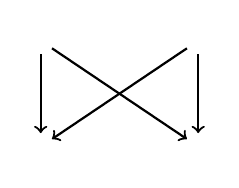
\begin{tikzpicture}
      \tikzstyle{every node}=[shape=circle];\path (0,0) node[below] (v0) {};\path (2,0) node[below] (v1) {};\path (0,1) node[above] (v2) {};\path (2,1) node[above] (v3) {};\draw[->, thick, black] (v2) -- (v1);\draw[->, thick, black] (v2) -- (v0);\draw[->, thick, black] (v3) -- (v1);\draw[->, thick, black] (v3) -- (v0);\end{tikzpicture}
  \end{center}
  where an arrow from  to  means  and if
   then either  or
  . This shows that the pair , 
  has no supremum and that the pair ,  has no
  infimum.\qed
\end{pf}


\subsection{Ideals and Filters}
\label{sec:idfi}

Although the structures  studied in this paper
are not semi-lattices (see above), many classical properties of
cellular automata are nicely captured through \emph{ideals} and
\emph{filters}. Well-known in lattice theory and algebra, the notions
of ideal and filter can also by defined for an arbitrary
(quasi-)ordered structure \cite{lattice}. For the structure
, an ideal  is a set of CA such that:
\begin{itemize}
\item if  and  then ;
\item for any  there is some  such that
   and .
\end{itemize}
Moreover,  is said \emph{principal} if there is some  such
that .  The notion of filter and
principal filter are dual of ideal and principal ideal (replacing all
 by ).

Given a set  of CA, the three following conditions are sufficient for
 to be an ideal for the simulation  (resp. , or
):
\begin{enumerate}
\item  for any transform ,
\item if  and  (resp. ,
  or ) then ,
\item if  and  then .
\end{enumerate}

Most of the proofs below follow this scheme.  

\subsubsection{Dynamical properties}

The following theorem shows that several dynamical properties of
global rules of CA correspond to ideals in the quasi-orders.  A CA is
nilpotent over periodic configurations if there exists a spatially
periodic configuration  such that all spatially periodic
configurations lead in finite time to .

\begin{thm}
  \label{thm:commonideal}
  Let  be a simulation relation among , 
  and . The following sets of CA form ideals of
  :
  \begin{itemize}
  \item surjective CA,
  \item reversible CA,
  \item CA which are nilpotent over periodic configurations.
  \end{itemize}
\end{thm}
\begin{pf}
  First, from the point of view of global maps, a geometric transform consists
  in iterating or composing with bijective maps. So the properties of being
  surjective or reversible are left unchanged by geometrical
  transforms. Besides, geometrical transforms map periodic configurations to
  periodic configurations, cycles of configurations to cycles of configurations
  (possibly reduced to a single configuration), and attraction basins of such
  cycles to attraction basins of cycles. Hence, nilpotency over periodic
  configurations, which is equivalent to the existence of a temporal cycle having
  all periodic configurations in its attraction basin, is preserved by
  geometrical transforms. By similar reasoning on the phase space, it is
  straightforward to check that  is nilpotent over periodic configurations
  if  is and  or . And 
  is nilpotent over periodic configurations if both  and  are. So
  nilpotency over periodic configurations induces an ideal for .

  It is also clear that surjectivity and reversibility are preserved
  by cartesian product. Now suppose . If  is
  surjective then so is  since
   and  is by
  definition surjective. If  is reversible, consider any map
   such that  and let  be the CA
  over state set  and defined by the global map  (it is a
  shift-commuting continuous map). Since
  , one can check that
   so  is reversible.
  
  Finally, suppose .  If  is reversible
  then  is also reversible since  and  is by definition
  injective. If  is surjective, then so is  because 
  being injective over finite configurations (Moore-Myhill
  theorem\footnote{In \cite{Hedlund:1969}, one can find the following
    theorem: a CA is surjective if and only if there is no pair of
    finite configurations (\textit{i.e.} uniform except on a finite
    region) having the same image. The original formulation of the
    Moore-Myhill theorem \cite{moore,myhill} supposes the existence of
    a quiescent state.})   is also injective over finite
  configurations ( maps finite configurations to finite
  configurations). \qed
\end{pf}

\begin{thm}
  Let  and  be two reversible CA and  be a
  simulation relation among ,  and
  . If  then
  .
\end{thm}
\begin{pf}
  First, it is straightforward to check that the inverse of
  geometrically transformed instances of  are transformed
  instances of the inverse of . Using what was shown above
  concerning reversibility, it is thus sufficient to prove the two
  following properties:
  \begin{itemize}
  \item  implies ,
  \item  implies .
  \end{itemize}
  In the first case we have:
   each
  equality being true on .  In the second case we have:
   each equality being true on
  .  \qed
\end{pf}

One immediate consequence of the theorem is that if two reversible CA
are equivalent then their inverse CA are also equivalent. What is not
obvious however is whether the inverse CA are necessarily in the same
class as the initial CA.

\begin{openpb}
  Consider any simulation relation and  the associated equivalence
  relation.  What are the reversible CA  such that ?
\end{openpb}

At the time of writing we have no example of a reversible  with
. 

\begin{thm}
  \label{thm:revuniv}
  Let  be  or . Then the ideal of
  reversible CA is principal: there is a reversible CA  such
  that
  
\end{thm}
\begin{pf}
  In \cite{DurandLose97}, a reversible CA  able to simulate any
  reversible CA is constructed. The notion of simulation used is
  included in  and therefore in . The
  implication  is thus proven and the converse
  implication is proven by theorem~\ref{thm:commonideal}.\qed
\end{pf}

For the ideal of surjective CA, the principality is still an open
problem in dimension 1.

\begin{openpb}
  \label{open:surjideal}
  Is the ideal of surjective CA principal, and for which simulation
  quasi-order?
\end{openpb}

Limit sets of CA have received a lot of attention in the literature
\cite{Culik89, hur87, goles93}. The limit set of  is the set
 of configurations having predecessors arbitrarily far in
the past, formally:


The next theorem shows that the class of CA with a sofic limit set is
nicely captured by .

\begin{thm}
  \label{thm:soficideal}
  The set of CA with a sofic limit set is an ideal for .
\end{thm}
\begin{pf}
  For CA of dimension 1, having a sofic limit set is equivalent to having a
  regular limit language \cite{weiss}. It is clear that this latter property is
  left unchanged by geometrical transforms (the limit language is not affected by
  iterations and shifts, the regularity of the language is not affected by
  packing). Hence, it is sufficient to show that if  has a regular limit
  language and  then  also has a regular limit
  language. Since regular languages are closed under substitution (a classical
  result which can be found in \cite{HopcroftUllam}), it is sufficient to prove
  that . This last assertion is
  a direct consequence of , since the following equality holds
  by recurrence on :
  \qed
\end{pf}

\begin{openpb}
  Let  be  or . Is there a -universal CA
  with a sofic limit set?
\end{openpb}

\subsubsection{Topological dynamics}

The properties considered above are purely dynamic: they can be
expressed as structural properties of the phase space with the
reachability relation only. We now consider properties from
topological dynamics: they are expressed with both the reachability
relation and the topology (Cantor distance) of the space of
configurations.  We will show that many of them correspond to ideals
of the simulation quasi-orders.

The properties we will consider are derived from the equicontinuity
classification of P.~K{\r u}rka \cite{Kurka97}. Let  be any CA
with state set  and global rule  and denote by  the
Cantor distance over .
\begin{itemize}
\item  is an \emph{equicontinuity point} for  if 
  
\item  is \emph{sensitive to initial conditions} if
  
\item  is \emph{(positively) expansive} if
  
\end{itemize}

The classification of P.~K{\r u}rka is the following:
\begin{description}
\item[] is the set of CA for which all configurations are equicontinuity points,
\item[] is the set of CA having equicontinuity points,
\item[] is the set of CA sensitive to initial conditions,
\item[] is the set of expansive CA.
\end{description}

The weakness of this classification is its lack of shift-invariance:
the identity and the elementary translation belong to different
classes ( and  respectively). Several attempts have been
made to overcome this problem by changing the topology \cite{besico}.
More recently, a new approach has been proposed \cite{sablikTCS}: the
Cantor topology is conserved (with all its good properties) but the
topological properties are enriched with a new parameter (a velocity)
which is used as the reference direction of information propagation in
space-time. The original definitions of P.~K{\r u}rka are thus
obtained by choosing velocity , but now identity and elementary
translations are assigned to the same class (with different
velocities). This directional dynamic approach is more suitable for
our study since, by definition, the equivalence classes of any of our
quasi-orders are shift-invariant. We will define  classes based on
the existence of some direction for which some dynamical behavior is
observed.

We say that  is a \emph{rescaling} of  if there are
transforms  and  such that
.  We then consider the
following  classes:

\begin{itemize}
\item the set  of CA which are a rescaling of some equicontinuous CA,
\item the set  of CA which are a rescaling of some CA having
  equicontinuity points,
\item the set  of CA which are not in , \textit{i.e.}
  CA which are sensitive in every directions\footnote{For
    one-dimensional CA, the set of sensitive CA is the complement of
    the set of CA having equicontinuity points (see \cite{Kurka97}). In
    \cite{sablikTCS}, this complementarity is shown for any
    direction.},
\item the set  of CA which are a rescaling of some
  (positively) expansive CA.
\end{itemize}

\begin{figure}[htbp]
  \centering
  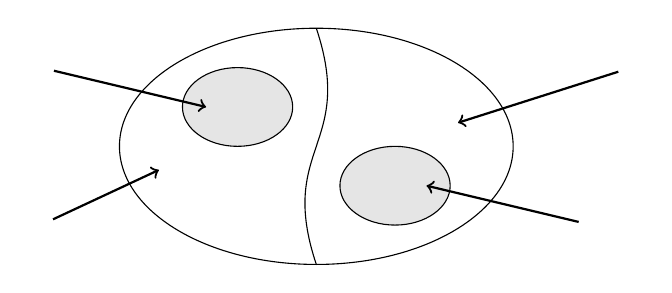
\begin{tikzpicture}
    \draw (0,0) ellipse (2.5 cm and 1.5 cm);\path (-1.1,-.8) node () {};\path (1.1,.8) node () {};\filldraw[fill=black!10, draw=black] (-1,.5) node (u) {} ellipse (.7cm and .5cm);
    \filldraw[fill=black!10, draw=black] (1,-.5) node (v) {} ellipse (.7cm and .5cm);
    \draw (0,1.5).. controls (.5,0) and (-.5,0)..(0,-1.5);
    \path (-3.5,1)  node[shape=circle] (id) {};
    \path (-3.5,-1)  node[shape=circle] (max) {};
    \path (4,1)  node[shape=circle] (sig) {};
    \path (3.5,-1)  node[shape=circle] (ztwo) {};
    \draw [->, thick] (id) -- (-1.4,.5);
    \draw [->, thick] (max) -- (-2,-.3);
    \draw [->, thick] (sig) -- (1.8,.3);
    \draw [->, thick] (ztwo) -- (1.4,-.5);
  \end{tikzpicture}
  \caption{Four kinds of topological dynamics.}
  \label{fig:shiftkurka}
\end{figure}

Figure~\ref{fig:shiftkurka} is justified by the following theorem.

\begin{thm} 
  We have the following inclusions:
  \begin{enumerate}
  \item ,
  \item .
  \end{enumerate}
  Moreover, each of the sets , ,
   and  is non-empty.
\end{thm}
\begin{pf}
  The first inclusion follows from definitions. The second follows
  from proposition 3.2 of \cite{sablikTCS} which asserts that the set
  of directions with equicontinuity points and the set of expansive
  directions cannot be simultaneously empty.

  Non-emptyness of  and  follows from the existence of
  equicontinuous (\textit{e.g.} the identity) and (positively)
  expansive CA (\textit{e.g.} ). Moreover, any CA having an
  equicontinuity point which is not equicontinuous (\textit{e.g.} the
  CA of local rule ) cannot be in
   (equicontinuity is preserved by rescaling), so it is in
  . Finally,
  . Indeed, for
  , any direction is either a direction of
  right-expansivity or a direction of left-expansivity, neither
  both. So . Finally,
   since, by proposition 3.2 of
  \cite{sablikTCS}, no direction of (left or right) expansivity can be
  a direction with equicontinuity points.\qed
\end{pf}

\begin{thm}
  \par\noindent
  \label{thm:tdideals}
  \begin{enumerate}
  \item  is an ideal for any simulation  among
    ,  and ;
  \item  is an ideal for ;
  \item  is an ideal for .
  \end{enumerate}
\end{thm}
\begin{pf}
  First, consider any . Then there are CA 
  and  which are both equicontinuous and -equivalent to
   and  respectively. Then, if 
  we have  and by theorem~\ref{thm:bfacts} we have
  both  and . The same reasoning can
  be applied to  and . Thus we have shown the
  second condition of the definition of ideals for the three properties
  considered here.

  To conclude the theorem, and since the three properties considered are
  by definition invariant by rescaling, it is sufficient to prove:
  \begin{itemize}
  \item if  or  then ;
  \item if  then ;
  \item if  then .
  \end{itemize}
  
  The first assertion follows from the characterisation of
  equicontinuous CA as ultimately periodic CA \cite{Kurka97}. 
  
  For the second assertion, if  then for all
   we have the inequality
  .  Moreover, for any
   there is some  such that
   and  (choose
   so that it equals  on the cells around position ).
  Hence, if  is an equicontinuous point for  then  is
  an equicontinuous point for .

  Finally, for the third assertion, it is sufficient to notice that
  the property of expansivity is defined by a formula using only
  universal quantifications on configurations so it remains true on a
  subset of configurations. \qed
\end{pf}

 is not an ideal for  and neither for
 as shown by the following example.
\begin{ex}
  Consider  of radius  and let  be the CA with
  radius , states set  (with ) with local rule  defined by
    so . However
   since the configuration  is
  an equicontinuous point.\qed
\end{ex}

Notice also that  cannot be an ideal because
 simulates .

\begin{openpb}
  \label{open:expansif}
  Are there  and  such that
   (\textit{i.e.} the simulator CA is expansive up
  to rescaling but the simulated CA is not expansive, even up to
  rescaling)?
\end{openpb}


\subsection{(Un)decidability}
\label{sec:undec}

The fact that many properties related to the simulation quasi-orders are
undecidable is no surprise. For instance the nilpotency property, which is an
undecidable problem \cite{kari92}, corresponds to an equivalence class in the
three quasi-orders (theorem~\ref{thm:nilper}). However, there are non-trivial
properties of these quasi-orders which are decidable (see below) and the edge
between decidable and undecidable properties is hard to catch.

In this section, we consider two kinds of problems in simulation
quasi-orders: lower bounds (being above some fixed CA or set of CA)
and upper bounds (being simulated by some fixed CA or some CA from a
fixed set).

\begin{thm}[\cite{mazrap}]
  The set of CA of radius  with a spreading state and nilpotent
  over periodic configurations is not co-recursively enumerable.
\end{thm}

\begin{thm}
  \label{thm:nilperdeci}
  Let  be any CA which is not nilpotent over periodic
  configurations. Let  be either  or
  . Then the set of CA  such that 
  is not co-recursively enumerable.
\end{thm}
\begin{pf}
  We describe a computable transformation which, given a CA  of radius 
  with a spreading state, produces a CA  with the following properties:
  \begin{itemize}
  \item if  is not nilpotent over periodic configurations then
    ;
  \item if  is nilpotent over periodic configurations then so is
    .
  \end{itemize}
  The theorem follows by theorem~\ref{thm:commonideal} since we have
  reduced the problem '?' to the problem of
  nilpotency over periodic configurations (reduced to CA of radius 
  with a spreading state).

  We now describe the construction of  from .  Suppose
   has a spreading state .  is the CA of radius  and
  states set 
  with local rule  defined by:
  
  where ,  and  represent component  of ,  and
  . Any periodic configuration  of  either leads to the
  uniform configuration , or contains a periodic
  configuration of  in its first component. Hence, if  is
  nilpotent over periodic configurations, then so is  (because
   is precisely the spreading state of ).  If  is not
  nilpotent over periodic configurations, then there is a word
   and an integer  such
  that the periodic configuration  of period  verifies
  . Therefore, by definition of , we have
   where
   is defined by:
  \qed
\end{pf}

This result shows that it is generally undecidable to know whether a
CA is lower-bounded by a given (fixed) one. However, there are
noticeable exceptions in one dimension for  and .

\begin{thm}
  \label{thm:abovenilpo}
  Let  be either  or  and let  be
  a nilpotent CA. Then the problem of determining if a given  is
  above  for  is decidable.
\end{thm}
\begin{pf}
  We are going to show that  if and only if  is
  not surjective and the theorem follows by decidability of
  surjectivity in one dimension \cite{amoroso72}.  First, by
  theorem~\ref{thm:commonideal}, if  is surjective then
  . Suppose now that  is not surjective,
  \textit{i.e.} that  possesses some Eden word 
  for some length . Then, denoting by  the CA over states set
   which is constant equal to , we have
   if
   verifies  if and
  only if . We deduce by theorem~\ref{thm:nilper} that
  .\qed
\end{pf}

\begin{openpb}
  \label{open:abovenilpo}
  Is there a non-surjective CA  which cannot injectively
  simulate any nilpotent CA? Is the problem of being above the class
  of nilpotent CA for injective simulation a decidable problem?
\end{openpb}


Concerning upper-bound problems, the edge between decidability and
undecidability is also non-trivial.  For instance,
theorem~\ref{thm:revuniv} shows the existence of a CA  such that
the upper-bound decision problem '?' is decidable in
dimension 1.


\section{Tops of the Orders}
\label{sec:top}

In this section we study maximal elements of the
quasi-orders. These CA are able to simulate any other CA

\begin{defn}
  Let  be any relation among ,  and
  . A CA  is said \emph{-universal} if for
  any  we have . It is \emph{strongly
    -universal} if it strongly -simulates any other CA.
\end{defn}

The notion of strong -universality above is exactly the same
notion as \emph{intrinsic universality} defined in section 5 of
\cite{bulking1} and has already been considered several times in the
literature (see \cite{JACsurvey} for a survey). In fact, strong and
general universality are the same notion for  and
.

\begin{thm}
  \label{thm:stronguniv}
  There exist strongly -universal CA and all
  -universal CA are strongly -universal. The same
  is true for .
\end{thm}
\begin{pf}
  For the existence of strongly -universal CA, see
  \cite{JACsurvey}. The theorem follows by application of
  theorem~12 of \cite{bulking1}. \qed
\end{pf}

Of course, any -universal is also
-universal. The converse is an open problem.

\begin{openpb}
  Do the notions of -universality and
  -universality coincide?
\end{openpb}


Concerning , the situation is different: no CA is strongly
-universal\footnote{The proof of this fact was suggested by
  G.~Richard.}.

\begin{thm}
  There is no strongly -universal CA.
\end{thm}
\begin{pf}
  Suppose for the sake of contradiction that there is some strongly
  -universal .  Consider a uniform configuration 
  of . There is  such that the orbit of  under 
  contains  different configurations (the orbit is ultimately
  periodic).  Now consider  with  states such that its
  uniform configurations are all in the same cycle of length .
  By hypothesis, for any  there is some geometric transform
   such that .  Let  be
  the corresponding configuration of  for
  . The orbit of  contains at most 
  different configurations and it is therefore the same for the orbit
  of  under . But  is necessarily uniform and we get
  a contradiction with the choice of . \qed
\end{pf}

The theorem 12 of \cite{bulking1} don't apply for . However,
we are not able either to construct a -universal CA, nor to
prove that there is none.

\begin{openpb}
  \label{open:surjuniv}
  Is there a -universal CA?
\end{openpb}

For the rest of this section, we consider only  and
.

\subsection{On the Way to the Top}
\label{sec:reachtop}

Universal CA are not hard to construct and the property of being
universal is recursively enumerable since simulation relations
considered here are recursively enumerable. However universality is
not co-recursively enumerable as shown by the following theorem. The
case of -universality was proven in \cite{Ollinger03}. Using
theorem~\ref{thm:nilperdeci}, the proof below is direct and includes
the case of .

\begin{thm}
  \label{thm:indeciuni}
  The set of -universal CA is not co-recursively enumerable
  and neither is the set of -universal CA.
\end{thm}
\begin{pf}
  There exists a CA which is -universal but not nilpotent
  over periodic configurations. To see this consider any universal CA
  and add a new state which is spreading: the resulting CA, say
  , contains at least two disjoint periodic orbits of periodic
  configurations and is thus not nilpotent over periodic
  configurations. The theorem follows by application of
  theorem~\ref{thm:nilperdeci} to  since  is by
  construction both -universal and
  -universal.\qed
\end{pf}

This result has some consequences on the structure of simulation
quasi-orders 'near' the top. The following theorem shows that a
non-universal CA is always 'infinitely far' from the class of
universal ones.

\begin{thm}
  \label{thm:notuniv}
  Let  be  or . And let  be the
  set of -universal CA. Then we have:
  \begin{enumerate}
  \item ,
  \item if  then there is  with
 but .
  \end{enumerate}
\end{thm}
\begin{pf}
  \par\noindent
  \begin{enumerate}
  \item By theorem~\ref{thm:bfacts} we have
     and  which
    proves one direction. Moreover, there exists  with
     states only \cite{banks,nicolasFCT}. If we suppose
     then, by theorem~\ref{thm:stronguniv},
    it strongly simulates . Hence, by theorem~\ref{thm:deprod},
    we have either  or  and thus
    either  or .
  \item Let . If  was such that
     for all  then the complement
    of  would be the set  and
     would be co-recursively enumerable contradicting
    theorem~\ref{thm:indeciuni}. So there is  with
    . To conclude the proof it is sufficient
    to choose  (theorem~\ref{thm:bfacts}).\qed
  \end{enumerate}
\end{pf}

\subsection{Necessary But Not Sufficient Conditions}
\label{sec:notuniv}

The purpose of this section is twofold. It compares the notions of
universality defined above to other definitions of the literature and,
by doing this, presents tools and techniques to prove non-universality
of some CA (other proofs of non-universality for other purposes are
developped in section~\ref{sec:io}). 

One of the techniques we use to ensure that some CA is not universal
yet achieving some behavior , is to add a spreading state and let
the CA generates this state if it detects somewhere that the current
configuration doesn't correspond to a 'legal' configuration,
\textit{i.e.} a configuration occuring normally when producing the
behavior .  Proofs of non-universality with this technique rely on
the lemma below. Before stating and proving the lemma, we need to give
some precisions on spreading states and sets of configurations
'supporting' a simulation.

First, the notion of spreading state is sensitive to the choice of the
syntactical representation of the CA because it depends on the choice
of the neihborhood. In the sequel we say a CA  has a spreading
state  if any cell changes to state  when 
appears in its minimal neighborhood (\textit{i.e.} the minimal set of
cells upon which the local rule effectively depends).

Second, given a relation of the form
, there is an isomorphism between
 and  as dynamical systems. At the level of
, the configurations involved in this relation is the set  of
configurations made of infinite concatenation of elements of
 (viewed as words of length  over
alphabet ). This kind of sets are called \emph{block-subshifts}
and discussed in more details in section 3.2 of \cite{bulking1}. In
the sequel, such a set  is called the \emph{support} of the
simulation.

\begin{lm}
  \label{lm:nospread}
  Let  be a CA without spreading state and  be a CA with a
  spreading state . If  strongly -simulates
  , then the support  of the simulation cannot contain
  .
\end{lm}
\begin{pf}
  By hypothesis, there are parameters , , ,  and a CA  such that
  
  By choice of ,  admits  as
  spreading state. Moreover, by definition of , the minimal
  neighborhood of  is included in the minimal neighborhood of
  . Thus, if  appears in some
  configuration of  then the state  is a
  spreading state for  because  also appears in 
  for arbitrarily large .\qed
\end{pf}



We first study how embeddings of Turing machines into CA can relate
the notions of universality for Turing machines to the notions of
universality derived from quasi-orders as defined above.

An embedding of a Turing machine  into a CA  is an
embedding of the instantaneous descriptions of  into
configurations of  such that instantaneous descriptions of
successive steps of  corresponds to successive steps of 
via the embedding. We don't give any formal definition of embedding
since we will never prove negative results (\textit{i.e.} assertions of
the form `there is no embedding of  such that...'). However, the
embeddings we use in the sequel are classical and already appeared in
the literature (see \cite{Sutner03}).

\begin{thm}
  \label{thm:embed}
  For any Turing machine , there exists a CA  which embeds
   but is not -universal.
\end{thm}
\begin{pf}
  Let  where  is the set of
  states of ,  is the tape alphabet, and  is
  the transition function of .  We construct a CA  over
  state set  where  and
   are states not already in . Each cell of 
  corresponds to a tape position of : it contains a letter from
  the tape alphabet and either a head with its current state or no
  head but an indication  or  telling in
  which direction to find the head. On configurations containing a
  single head,  mimics transitions of  step by step as
  expected. Thus,  embeds . In addition,  checks
  that  a never occur to the left of a state from 
  or a  (and symmetrically for ). If the
  check fails, then the state  is generated and spreads.

  This construction ensures that, for any initial configuration ,
  if the orbit of  never contains an occurrence of  then it
  contains at most one head. Hence, these orbits are such that at any
  time step state changes occur on the neighborhood of at most one
  position (a head move involves a state change in two adjacent
  cells).

  Now suppose that  is -universal and consider the
  CA .   strongly simulates
   (theorem~\ref{thm:stronguniv}).  Since  has no
  spreading state, then the set  of configurations of  on
  which the simulation occurs never contains . We deduce that
  all orbits of configurations from  have the property described
  above. This implied that  is such that on all its orbits, at
  most two cells change their states between two steps: this in
  contradiction with the choice of .\qed
\end{pf}

Turing-universality of cellular automata is a fairly vague notion in
the literature. We don't give a formal definition here since we won't
prove any negative result concerning Turing-universality. We just
consider that a CA able to embed a universal Turing
machine\footnote{We don't give any formal notion of universality for
  Turing machine either. In fact, we only need to suppose the
  existence of at least one universal Turing machine.} is
Turing-universal.

We can choose  to be universal in the previous theorem
(theorem~\ref{thm:embed}). In this case, since the embedding used in
the proof ensures that  is simulated in real time by , we
deduce that the following problem is P-complete:
\begin{description}
\item[Input:] a state , an integer , and a
  word  where  is the radius of ;
\item[Query:] do we have ?
\end{description}
This problem of finite triangle computation has been considered
several times in the literature and it has been proven that it was
P-complete for particular CA \cite{GriffeathMoore, NearyW06}.  This
notion of complexity inherited from sequential computation theory
fails to capture the notion of universality associated to simulation
quasi-orders.

\begin{cor}
  There exists a CA which is Turing-universal and P-complete but not
  -universal.
\end{cor}


\section{Induced Orders}
\label{sec:io}

This section aims at studying particular CA or sets of CA for the
ordered structure they induce in the simulation quasi-orders.  While
studying various properties of the quasi-orders in the previous
sections, we have already established the existence of several induced
infinite structures.

For instance, theorem~\ref{thm:notuniv} allows to construct an
infinite strictly increasing chain of non-universal CA starting from
any non-universal CA for the quasi-orders associated to  and
.  Besides, theorem~\ref{thm:shishi} implies the
existence of inifinite chains in the three quasi-orders studied in this
paper.

Section~\ref{sec:limprod} below gives a way to construct chains of
length  and an hint about the existence of chains of
length . However, we leave open the question of
the longest chain induced in any of the quasi-orders. We don't even
know if one of them admits a dense chain.

\begin{openpb}
  Does one of the quasi-orders admit a dense induced order?
\end{openpb}

\subsection{Limit Cartesian Product}
\label{sec:limprod}

We have seen in theorem~\ref{thm:notuniv} that if  is not
universal, then  cannot be universal. Therefore, no
finite Cartesian product of  with itself can be
universal. Therefore, we have a chain of non-universal CA:

For some , the chain collapses in a single equivalence class,
\textit{e.g.} if  is a translation (see
lemma~\ref{lm:canoshi}). However, the following theorem shows that for
some , the chain is strictly increasing. Moreover,  can be
chosen so that it embeds any Turing machine. 

\begin{thm}
  \label{thm:turingheads}
  For any Turing machine , there is a CA  which embeds
   and such that for any , one has:
  
\end{thm}
\begin{pf}
  Le  be the CA constructed in the proof of
  theorem~\ref{thm:embed}. We can suppose that  is such that it
  can produce infinite sequences of left move of its head when started
  from a special state (not the initial state) over a blank tape, and
  more precisely that the sequence of moves leaves the tape blank.  If
   does not have this property, just add some states to achieve
  this behavior. We can suppose the same for right moves.
  
  Denote by  the product of  copies of  and by
   the product of  copies. Suppose for the sake of
  contradiction that . We can construct
  for any set of positions  a configuration  of
   such that for all  the th component contains a
  correct instantaneous description of  where the head is at
  position  in a state suitable to generate an infinite sequence
  of left or right moves (as supposed above).  Now let  be a
  configuration of  corresponding to  via
  simulation. First, if some component  of  contains a
  spreading state, it will spread and, after some time , will be
  present at some position where the configuration
   contains no head, but only a blank tape symbol
  on each component. This means that blocks of blank tape symbols in
   can be simulated by blocks of  where the th
  component is a block of spreading states. Considering again the
  orbit of , we deduce that it can be simulated by a configuration
   where the th component is everywhere a spreading state
  except at a finite number of positions. Thus after some time, the
  th component will become uniform and constant. It is then
  straightforward to show that it is useless for the simulation and
  that in fact  on  can be simulated by only  copies
  of .

  Applying the reasoning inductively, we can therefore suppose that no
  spreading state appears on any component in the orbit of the
  configuration  defined above. Since, the orbit of  is such
  that there are  distant positions where some states change at each
  step, it must be the case in the orbit of . Since, ,
  there must be some component with two heads and therefore a
  spreading state must appear after the first step: this is in
  contradiction with what we have just supposed.\qed
\end{pf}

For the CA  of the previous theorem, we can ask if the infinite
chain of Cartesian products is upper-bounded by some non-universal CA, or
if any CA able to simulate each product of the chain is necessarily
universal. One can imagine that for a sufficiently simple ,
there is some room above the chain of products of  and below the
class of universal CA.

The rest of this section is devoted to the proof of a stronger result:
for any , there is a CA  which is able to simulate any
finite product of  and such that  is universal if and only
if  is universal. Moreover,  can be obtained from 
constructively. Because it extends property of Cartesian product given
by theorem~\ref{thm:notuniv}, this construction will be called
\emph{limit product} in the sequel. If  is a CA, its limit
product is denoted by .

\textit{Note: }In the rest of this section we only consider the
simulation . 


Without loss of generality, we can suppose that  has radius 
(theorem~\ref{thm:bfacts}). To be able to simulate the product 
of  copies of ,  is made of three layers (its
state set is a Cartesian product union a single state, which is a
spreading state as explain hereafter):
  \begin{enumerate}
  \item the \emph{state} layer,
  \item the \emph{transport} layer, and
  \item the \emph{synchronisation} layer.
  \end{enumerate} It proceeds as follows.
\begin{description}
\item[State layer.] Each component of a cell of  is simulated by a block of
  three adjacent cells in the state layer of .  More
  precisely, component  () of cell  of 
  is simulated by the block of three cells of  beginning
  at position . This block is referred to as  in
  the sequel. In , the center cell stores the th
  component of the cell  of  and the two other are used to
  store temporarily the th components of cell  and .
\item[Transport layer.] The role of the transport layer is precisely to bring states of
  th components corresponding to cell  and  of  to
  the dedicated cells of  in . Then, the
  transition  of the th component of
   can be simulated locally by  in
  . Transport is done in parallel for any  and any
  . To do this, the transport layer is made of a succession of
  particles (one every three cells), each one being able to carry a
  state of . Initially aligned with the center of blocks, the
  particles move in parallel according to a cycle of five steps:
  \begin{enumerate}
  \item move right by  cells and read the state seen on the state layer;
  \item move left by  cells and write the memorized state on
    the state layer;
  \item move left by  cells and read the state seen on the state layer;
  \item move left by  cells and write the memorized state on
    the state layer;
  \item move  cell right and apply local rule  on state
    layer at the current position;
  \end{enumerate}
\item[Synchronisation layer.] The role of the synchronisation layer is
  to orchestrate the cycle of particle moves and it must be able to do
  it for arbitrary large values of  (simulating arbitrarily large
  Cartesian products of  is sufficient to simulate all products
  of ). It contains a flag that can take one of the four
  indications 'left', 'right', 'read', 'write' and 'transition'. The
  flag is changed everywhere synchronously according to a cycle
  suitable to ensure that particles of the transport layer produce the
  cycle described above when they follow the instruction given by the
  flag.
\end{description}

We now describe in detail the synchronisation layer.  Denote by
 the flag sequence mentionned above in the simulation of
a product of  copies of , and let  be the set of flag
states.

\begin{thm}
  \label{thm:metronome}
  There is a CA  with a spreading state  and a map  such that  is not
  -universal, and, for any configuration
  , one of the following property is true:
  \begin{description}
  \item[Cycle:] at each time in the orbit of , all cells have the
    same image by  and the sequence with time of this common
    image is periodic of period  for some ;
  \item[Frozen:] at each time in the orbit of , all cells have the
    same image by , but this common image remains constant after
    a certain time;
  \item[Error:] the spreading state appears at some time in the orbit
    of .
  \end{description}
  Moreover  is such that there are configurations having the
  'cycle' property above producing period  for
  arbitrarily large .
\end{thm}
\begin{pf}
  First, notice that flag changes in the sequence  are
  separated by a number of steps which is either constant (independant
  of ), or of the form  with  a constant (we can suppose
   without loss of generality). To simplify notations, we
  will suppose in this proof that  alternates between two
  values  and  every  steps. Adapting the proof for the
  real  is just a matter of adding a finite set of
  special states to deal with constants.
  
  The proof is based on a reversible solution  to the firing
  squad synchronization problem proposed by K.~Imai and K.~Morita: in
  \cite{ImaMor96}, they construct a reversible CA  with a
  subset of states  (the firing states) such that for any ,
  there is a periodic configuration  verifying\footnote{In
    \cite{ImaMor96}, the main concern is synchronisation of finite
    segments of cells surrounded by a quiescent state. To extend the
    property to infinite configurations, it is crucial that
    ``garbage'' (which must be conserved to ensure reversibility) do
    no spread outside the initial segment. The solution of K.~Imai and
    K.~Morita has precisely this property as it is explicitely
    mentionned in \cite{ImaMor96}.}:
  \begin{itemize}
  \item 
  \item  for all ,
    .
  \end{itemize}
  
  Without loss of generality, we can suppose that  and its
  inverse are syntactically represented with the same radius.  We now
  define a CA  of radius , with states set
  , and with
  transition function:
  
  where  equals  if  and  else. Intuitively, on
  configurations where the third component is uniform equal to , 
  mimics  on the first component and  on the second one if
   or the converse if . Moreover, the value of  is switched
  each time the component playing  encounters a firing state. Hence, if we
  choose for  the projection on third component,  started from
  configurations  has the property 'cycle' and produces the periodic
  sequence .

  We now enrich  with a spreading state which is produced each
  time one of the following local checking fails:
  \begin{itemize}
  \item the third component  must be uniform;
  \item for the two first components, a state from  (firing state)
    must always be surrounded by states from  only;
  \item states from  are forbidden on the second component if
     and states from  in the first component are forbidden
    if .
  \end{itemize}
  The third condition ensures that in the case of a 'cycle' regime
  (firing states appearing infinitely often), the period is equally
  divided between steps where  and steps where . To
  ensure that such a 'cycle' regime always produces an alternance of
  exactly  zeros and  ones, we add a component implementing a
  counter modulo : the value of this component is incremented modulo
  3 at each step (whatever the context) and a spreading state is
  generated if a cell contains a firing state and the counter is not
   modulo . Denote by  the CA obtained and consider any
  configuration . If no spreading state appears in the orbit of
  , then the third component is uniform. If it changes of state
  only a finite number of times, then we are in the 'frozen'
  regime. If there are infinitely many changes, it follows from the
  discussion above that the conditions of the 'cyclic' regime are
  fulfilled.

  To conclude the theorem, it remains to prove that  is not
  -universal. Suppose for the sake of contradiction that it is and
  let  be any universal CA without spreading state and consider the set
   of configurations of  which is the support of the strong simulation
  of  ( strongly simulates  by
  theorem~\ref{thm:stronguniv}).  cannot contain any occurrence of the
  spreading state (by lemma~\ref{lm:nospread}), it implies that all
  configurations of  have a uniform third component. But, on such
  configuration, the dynamics of  is reversible. Hence  is
  reversible: this is a contradiction with its universality by
  theorem~\ref{thm:commonideal}.\qed
\end{pf}

The synchronization layer of limit products is exactly the automaton
 of the previous theorem, except that the spreading state of
 now becomes a global spreading state.  Before establishing the
main result of this section, we give more details concerning the state
layer and the transport layer of .

The state layer is made from state set  where
,  and  are states to identify explicitly the role of each
cell in each block :  for the cell storing the th
component of cell  of  and  and  to temporarily store
states of th component of cells  and  respectively.

The transport layer is made from state set 
where  is the state used to separate particle carrying a state
from .

So the states set of  is:
 

In addition to the behavior described above,  does the
following local checkings and generates the spreading state 
if one of them fails:
\begin{itemize}
\item the second component of transport layer must be periodic of period ;
\item the transport layer must contain an alternance of one state from
   and two states ;
\item when doing read and write operations, the particles of the
  transport layer must be aligned with the right type of state in the state layer:
  \begin{itemize}
  \item type  when reading,
  \item type  when writing at step ,
  \item type  when writing at step ;
  \end{itemize}
\item when the synchronisation layer says 'transition', check that the
  particules are aligned with cell of type  in the state layer.
\end{itemize}

All those checkings ensure the following property: if no spreading
state is generated and if the component layer produces a correct cycle
of instructions, then the behavior of the state layer is equivalent
to the behavior of some Cartesian product of  (up-to some
rescaling).

Before stating the main theorem, we establish a simple yet useful
lemma saying that if  simulates  with support , then
everything  can simulate using a support included in  can
also be simulated by .


\begin{lm}
  \label{lm:lift}
  Let  be either  or .  Let  and
   be such that the simulation  occurs on a
  support  of configurations of . If  -simulates
   on a support included in , then  -simulates
  .
\end{lm}
\begin{pf}
  We consider the case where  is .  By hypothesis, we
  have  on support
   and  on support
  . Now, let , , 
  and  be the packing parameters of transforms ,
  ,  and  respectively. The injective maps
   and  induce two injective maps  and
   with the following domains and ranges:
  
  Therefore  is a
  well-defined injective map from  into
  . Now define the transforms 
  and  to be the composition of  and , and of
   and  respectively. Then we have
  .

  The extension of the previous reasoning to  is
  straightforward.  \qed
\end{pf}


This lemma together with lemma~\ref{lm:nospread} is the key to a kind
of 'self-checking' simulation used in the construction of the limit
product (and re-used in section~\ref{sec:fam}). A 'self-checking'
simulation of  by  is standard simulation of  by
 on some support  with the additional property that 
'checks' locally on any configuration that it belongs to , and
triggers some pathological behavior (typically a spreading state) in
case of check failure.  Hence any possible strong simulation of some
 by  is such that:
\begin{itemize}
\item either it has a support included in  in which case  can
  also simulate  by lemma~\ref{lm:lift},
\item or it must contain some  in its support in which
  case a spreading state is generated and lemma~\ref{lm:nospread}
  gives some limitation on .
\end{itemize}

To show that a spreading state is generated in the second case above,
a crucial property is that the support of any simulation is by
definition always irreducible: if  and  are words occuring
in two configurations of the support, there exists a third
configuration of the support where  and  both appear (see
section 3.2 of \cite{bulking1} for a more detailed discussion on
supports of simulations).

We now state the main theorem of this section.

\begin{thm}
  \label{thm:limprod}
  For any , its limit product  is such that:
  \begin{itemize}
  \item  for all ,
  \item  is -universal if and only if
     is -universal.
  \end{itemize}
\end{thm}
\begin{pf}
  The first assertion follows from the construction of  and the
  detailed discussion above. Now suppose that  is
  -universal and let  be any universal CA with no spreading
  state. By theorem~\ref{thm:stronguniv},  strongly simulates
  :  for some geometrical
  transform . Let  denote the support of the simulation. By choice of
  , the spreading state  cannot appear in any orbit of any
  configuration of  (by lemma~\ref{lm:nospread}). We deduce from
  theorem~\ref{thm:metronome} that the synchronization component is in the same
  regime (either 'cycle' for a fixed value  or 'frozen') for all the
  configurations of  because otherwise, we could construct a configuration in
   producing a spreading state (by irreducibility of ).

  In the case where all configurations are in the frozen regime, the
  flag of the synchronization layer becomes constant after some time
  , so the transport layer has the behavior of a translation (or
  identity) and the state layer remains constant.  is identical
  for all configurations of  (because otherwise, we could once more
  combine two configurations to produce a spreading state, by
  irreducibility of ). Then, consider a CA  with state set
   which has the following
  behavior:
  \begin{itemize}
  \item the second component is decreased by one until it reaches ;
  \item on the first component, the local rule of  is applied,
    but only if the second component is .
  \end{itemize}
  Since  is -universal, it can strongly simulate
   (by theorem~\ref{thm:stronguniv}): precisely,
  . Consider the set  of
  configurations of  corresponding via simulation to the set of
  configurations of  uniformly equal to  on the second
  component. Denote by  the corresponding set of
  configurations of . By choice of , we know
  that  simulates itself on the set of configurations
  . This implies that for some ,  can simulate  using as support the set
  of configurations . By hypothesis,
  starting from such configurations,  has a behavior
  of translation or identity on the state and transport layers. Since
  the synchronizing component evolves independently of the others, we
  deduce by lemma~\ref{lm:lift} that there is some CA  which is
  a product of translations (corresponding to state and transport
  layers) such that  simulates : this is a
  contradiction by theorem~\ref{thm:notuniv} since neither 
  (theorem~\ref{thm:shishi}), nor 
  (theorem~\ref{thm:metronome}) is universal.

  Hence, we are necessarily in the case where the synchronization
  layers produce a valid cycle. Since no spreading state can be
  generated in the orbit of any configuration of , the state layer
  always behaves like a Cartesian product of  copies of . The
  value of  is in fact common to all configurations of  (as
  shown above), so we deduce by lemma~\ref{lm:lift} that
   simulates  and
   is therefore universal by theorem~\ref{thm:notuniv}. \qed
\end{pf}

Of course, we can consider  itself as a new candidate
for taking its finite Cartesian products and applying the limit
product construction. In fact, the process can be repeated forever
with the guarantee that no CA ever produced in this chain will be
universal, provided the initial CA is not. However, there is no reason
why this infinite chain should be strictly increasing. In particular,
even if

is a strictly increasing chain, it might be the case that
 is equivalent to
. Therefore we have only proven
that one of the following properties is true:
\begin{itemize}
\item there is a strictly increasing chain of length
   in the quasi-order ,
\item for any non-universal CA , there is a non-universal CA
   such that  and  is
  equivalent to .
\end{itemize}

\subsection{Sub-Families of Cellular Automata}
\label{sec:fam}

Theorem~\ref{thm:bfacts} shows that any equivalence class in any
quasi-order contains some CA with radius . This fact is a direct
consequence of a well-known transformation of CA with large radius
into CA of smaller radius with more states (this transformation is
called 'higher block presentation' in symbolic dynamics,
see~\cite{LindMarcus}).

It is also sometimes invoked in the literature that considering CA
with two states only is not restrictive since there is a converse
transformation that transforms a CA with many states into a CA with
only two states but a larger radius. However, the situation is not
similar to that of radius reduction since there are equivalence
classes with no -states CA: \textit{e.g.}   for any prime
 as shown by theorem~\ref{thm:mazrapadd} and
lemma~\ref{lm:manulem}. Note that the same is true for any fixed state
set of cardinal : the equivalence class of  contains no
such CA provided  is prime and does not divide .

Hence, this transformation introduces a bias: the transformed CA may
be inequivalent to the original one. Meanwhile, we know that CA with
two states can be as powerful as CA in general since there are
universal CA with two states only \cite{banks,nicolasFCT} (for
simulation relations  and ). More precisely, as
we will see below, the transformation applied to a universal CA always
yields a universal CA because the transformed CA simulates the
original one. Since the original and the transformed CA are not always
in the same equivalence class, one question that naturally arises is:
what CA can be simulated by the transformed CA but not by the original
one?  Although it provides only partial answers, this section is
devoted to that kind of questions, for CA with two states and for
other families.

Formally, given a familly  of CA, we say that a map
 is a -encoding of CA into familly
 if

We will only consider simulation relations  and  in the
sequel, thus an encoding into  implies that there are universal CA in
. A trivial example of such an encoding is given by 
where  is a universal CA and  is the function mapping any CA to
.  We are interested in using this notion of encoding with families which
are more 'representative' of the diversity of behaviors in the whole set of CA.
To express this we introduce the following notion of \emph{faithfulness}.

Given a -encoding  and a set  of
CA, we say that  is \emph{faithful} for  if:

An encoding is faithful for  if the original CA and its image by
the encoding simulate exactly the same CA in . So, to give some
evidence that a family  is 'representative' of CA in general,
we can exhibit an encoding of CA into  which is faithful for a
set  of CA as large as possible. When  is the whole set of CA,
the faithfulness implies that there is a CA of family  in any
equivalence class: this is the case for CA with radius .\\

The next theorem gives four encodings which are faithful for , the
set of -universal CA. The families corresponding to these
encodings were already defined in this paper except one: captive CA.

Captive CA were introduced in \cite{Theyssier04} and are defined by a
simple restriction on the transition rule. A CA , with state set
, radius  and local rule  is captive if:


In the following theorem, encodings are different but their
faithfulness rely on the same idea of 'self-checking' simulation
explained above which uses lemma~\ref{lm:nospread} and
lemma~\ref{lm:lift}.

\begin{thm}
  \label{thm:encodings}
  Let  be  or .  For any family of CA
  below, there is a -encoding from CA into  wich is
  faithful for the set  of -universal CA:
  \begin{itemize}
  \item CA with two states,
  \item CA in ,
  \item CA in , 
  \item captive CA.
  \end{itemize}
\end{thm}
\begin{pf}
  To describe the encoding for each family, we suppose  is a CA
  with state set , with radius  and
  location rule .
  \begin{description}
  \item[-states CA.] Let  be an integer large enough and 
    be an injective map from  to  such that no
    word  contains an occurrence of . Now define the
    injective map  by
    . Let .  is a
    CA of radius  and state set  defined as follows:
    \begin{itemize}
    \item on the set  of configurations made of infinite
      concatenations of words from ,  is
      isomorphic to  so that ;
    \item everywhere else,  generates a .
    \end{itemize}
    The map  is thus an encoding of CA into -states CA. Now
    suppose that  is universal and let  be a
    universal CA with two states and no spreading state which is
    strongly simulated by  on support 
    (theorem~\ref{thm:stronguniv}). If there is some  with
     then
    \begin{itemize}
    \item either there are two occurrences of  in  which are
      not correctly spaced,
    \item or there is a word  occurring in  with
      .
    \end{itemize}
    In any case, the image of  will contain an occurrence of 
    (because the above error must be seen by at least three consecutive
    cells) and 's will propagate like a spreading state which is
    impossible by lemma~\ref{lm:nospread} because otherwise
     could simulate  on a support
    where it possesses the spreading state . So 
    and lemma~\ref{lm:lift} shows that  simulates . Hence
     is universal if and only if  is.

  \item[Captive CA.] The encoding technique for captive CA is very
    similar and already appeared in a non-faithful form in
    \cite{Theyssier04}. Let  be the word , let
     be a state not in  and denote
    . We define the injective map
     by . We then
    define  in a way similar to the case above. Its radius
    is , its state set is  and its local rule is
    such that:
    \begin{itemize}
    \item on the set  of configurations made of infinite
      concatenations of words from ,  is
      isomorphic to  so that ;
    \item everywhere else,  take as new state the maximum
      of its neighbors for some fixed ordering of  such that 
      is the maximum.
    \end{itemize}    
    First,  is captive and  defines an encoding of
    CA into captive CA. Second, notice that for any support of
    simulation  of , if there is some  with
     then, by irreducibility of , either there is
     with  and  contains a , or 
    never appears in . In the second case,  always
    applies a  as local rule and therefore possesses a spreading
    state when restricted to . In the first case, consider the
    configuration  and  such that positions  and
     both see a  in their neighborhood and a local pattern
    not in  (such a  must exist by choice of  and definition
    of ). Then  contains the pattern  which
    is spreading by definition of . In any case we can
    apply the usual reasoning with lemma~\ref{lm:nospread} and
    lemma~\ref{lm:lift}: any CA without spreading state strongly
    simulated by  is also simulated by . So the
    encoding  is faithful for universal CA.
  \item[ and .] For , the encoding is
    simple:  is just  with an additional state
     which is spreading. The resulting CA  is
    always in  since  is a blocking word (see
    \cite{Kurka97}). Lemma~\ref{lm:nospread} is then sufficient to
    prove that it is an encoding from AC to  which is faithful
    for universal CA.

    For , the proof is even simpler:
     is always in
     since  and an
    equicontinuous point in a Cartesian product induce equicontinuous
    points for each component.  Theorem~\ref{thm:notuniv} concludes
    for the faithfulness.
  \end{description}
  \qed
\end{pf}

These encodings allow to transport some properties of general CA
concerning the top of quasi-orders into order structures induced by
each family\footnote{A stronger result concerning captive CA appears
  in \cite{Theyssier05}: -universality is undecidable even if
  we restrict to captive CA with a fixed (but sufficiently large)
  radius.}.

\begin{cor}
  Let  be  or  and let  be a
  family of CA among: CA with two states, , , captive
  CA.  Then we have the following properties:
  \begin{itemize}
  \item the set of -universal CA in  is not co-r.e.
  \item for any non-universal , there is a non universal
     with  but .
  \end{itemize}
\end{cor}
\begin{pf}
  The first property is a direct corollary of
  theorem~\ref{thm:encodings} and~\ref{thm:indeciuni} by definition of
  faithful encodings.

  For the second property, consider the encoding  established in
  theorem~\ref{thm:encodings} and let  be any
  non-universal CA. By theorem~\ref{thm:notuniv}, there is some
  non-universal CA  such that  but
  . By faithfulness of ,
   is not universal and by the definition of
  encoding it simulates  without being simulated by .\qed
\end{pf}

The families considered above induce structures sharing some
properties with the general quasi-orders 'near the top'. However, the
complete characterisation of equivalence classes occupied by some CA
of these families is more challenging.

\begin{openpb}
  What are the quivalence classes of the simulation quasi-orders
  containing a -states CA? a captive CA? a CA from ? a CA
  from ?
\end{openpb}

\section{Summary of results}

Figures~\ref{fig:injbulking}, \ref{fig:surjbulking} and \ref{fig:mixbulking}
hereafter give a summary of results and open problems concerning each of the three
quasi-orders studied in the paper.









\newcommand\class[2]{\draw[fill=white] #1 circle (.47cm);\draw #1 node {#2};}

\newcommand\coolclass[2]{\draw #1 node[ellipse,fill=white] {#2};}

\newcommand\simlink[2]{\draw #1 -- #2;}

\newcommand\dontknow[2]{\draw #1 node[ellipse,draw,fill=gray!20] {#2};}

\newcommand\thmref[3]{\path #1 -- #2 node[sloped,above,pos=0.40] {#3};}

\newcommand\lebas{(1,0)}
\newcommand\univcls{(3,15)}
\newcommand\runiv{(-.8,7)}
\newcommand\topsurj{(-1.8,10)}
\newcommand\topexp{(-3.3,5.3)}
\newcommand\zpz{(-3.5,2)}
\newcommand\zdz{(-2,2)}
\newcommand\nilpo{(7.5,2)}
\newcommand\iden{(2.4,2)}
\newcommand\sudt{(1.5,3.2)}
\newcommand\sudq{(0,3.2)}
\newcommand\sudtq{(.4,4.6)}
\newcommand\sudtc{(-1.1,4.6)}
\newcommand\turuniv{(6,6)}

\newcommand\surjgauche{(-6,1)}
\newcommand\surjdroite{(5,2)}
\newcommand\revgauche{(-2.2,4.3)}
\newcommand\revdroite{(4,2)}
\newcommand\expgauche{(-4.7,1.5)}
\newcommand\expdroite{(-1,2)}
\newcommand\expbas{(-2,.7)}

\thispagestyle{empty}


\begin{figure}
  \hskip -2cm\hbox{\begin{tikzpicture}
\draw[bottom color=yellow!80,top color=yellow!10] \lebas..controls
    \surjgauche..\topsurj..controls \surjdroite..\lebas;
\draw[bottom color=orange!80,top color=orange!10] \lebas..controls
    \revgauche..\runiv..controls \revdroite..\lebas;
\draw[bottom color=red!80,top color=red!10] \expbas..controls
    \expgauche..\topexp..controls \expdroite..\expbas;

\draw[dotted] \zpz++(-1.5,0)--(9.5,2);


\thmref{(8.5,2)}{(9.5,2)}{\small level 1}
    \thmref{\topsurj}{\surjgauche}{\tiny Surjective ideal, Thm. \ref{thm:commonideal}}\thmref{\runiv}{\revdroite}{\tiny Reversible ideal, Thm. \ref{thm:commonideal}}\thmref{\sudtc++(0,.5)}{+(1,0)}{\tiny Thm. \ref{thm:noshishi}}\thmref{\univcls++(-.5,.5)}{+(1,0)}{\tiny Thm. \ref{thm:stronguniv}}\thmref{\topexp}{\expgauche}{\tiny Thm. \ref{thm:tdideals}}\thmref{\topexp}{\expdroite}{\tiny Expansive ideal}\coolclass{\univcls++(0,-2)}{\tiny Thm. \ref{thm:notuniv}}\thmref{\lebas}{\zpz}{\tiny Thm. \ref{thm:zpz}}\thmref{\runiv++(0,.5)}{+(-1,0)}{\tiny Thm. \ref{thm:revuniv}}\thmref{\iden}{\lebas}{\tiny Thm. \ref{thm:nilper}}\thmref{\lebas}{\nilpo}{\tiny Thm. \ref{thm:nilper}}\thmref{\turuniv++(0,1)}{+(0,2.5)}{\tiny Thm. \ref{thm:turingheads}}

\dontknow{\topsurj}{\small Open Pb. \ref{open:surjideal}}\dontknow{\topexp}{?}\dontknow{(5.2,2)}{\small Open Pb. \ref{open:abovenilpo}}

\simlink{\lebas}{\zpz}\simlink{\lebas}{\zdz}\simlink{\lebas}{\iden}\simlink{\lebas}{\nilpo}\simlink{\iden}{\sudt}\simlink{\iden}{\sudq}\simlink{\sudt}{\sudtq}\simlink{\sudt}{\sudtc}\simlink{\sudq}{\sudtq}\simlink{\sudq}{\sudtc}\foreach \i in {-3,-1,1,3} \draw[dashed] \univcls--+(\i,-2.5);\draw[dashed] \nilpo--+(-2,2);\draw[dashed] \nilpo--+(2,2);\simlink{\turuniv}{+(0,1)}; \draw[dashed] \turuniv++(0,1)--+(0,2);

\coolclass{\turuniv}{ (Turing-universal)}\coolclass{\turuniv+(0,1)}{}\coolclass{\turuniv+(0,3.5)}{}\class{\lebas}{}\class{\univcls}{U}\class{\runiv}{RU}\class{\zpz}{\small}\class{\zdz}{\small}\class{\nilpo}{NIL}\class{\iden}{}\class{\sudt}{\tiny }\class{\sudq}{\tiny }\class{\sudtq}{\tiny }\class{\sudtc}{\tiny }\end{tikzpicture}}
  
  \caption{Injective bulking (quasi-order )}
\label{fig:injbulking}
\end{figure}

\begin{figure}
  \hskip -2cm\hbox{\begin{tikzpicture}
    \begin{scope}
\draw[bottom color=yellow!80,top color=yellow!10] \lebas..controls
      \surjgauche..\topsurj..controls \surjdroite..\lebas;
\draw[bottom color=orange!80,top color=orange!10] \lebas..controls
      \revgauche..\runiv..controls \revdroite..\lebas;
\draw[fill=gray!20] \expbas..controls \expgauche..\topexp..controls
      \expdroite..\expbas;

\draw[dotted] \zpz++(-1.5,0)--(9.5,2);


\thmref{(8.5,2)}{(9.5,2)}{\small level 1}
      \thmref{\topsurj}{\surjgauche}{\tiny Surjective ideal, Thm. \ref{thm:commonideal}}\thmref{\runiv}{\revdroite}{\tiny Reversible ideal, Thm. \ref{thm:commonideal}}\thmref{\sudtc++(0,.5)}{+(1,0)}{\tiny Thm. \ref{thm:noshishi}}\thmref{\univcls++(-.5,.5)}{+(1,0)}{\tiny Thm. \ref{thm:stronguniv}}\thmref{\topexp}{\expgauche}{\small Open Pb. \ref{open:expansif}}\thmref{\topexp}{\expdroite}{\tiny Set of expansive CA}\coolclass{\univcls++(0,-2)}{\tiny Thm. \ref{thm:notuniv}}\thmref{\lebas}{\zpz}{\tiny Thm. \ref{thm:zpz}}\thmref{\runiv++(0,.5)}{+(-1,0)}{\tiny Thm. \ref{thm:revuniv}}\thmref{\iden}{\lebas}{\tiny Thm. \ref{thm:nilper}}\thmref{\lebas}{\nilpo}{\tiny Thm. \ref{thm:nilper}}\thmref{\turuniv++(0,1)}{+(0,2.5)}{\tiny Thm. \ref{thm:turingheads}}\thmref{\turuniv++(0,3.5)}{+(0,2.5)}{\tiny Thm. \ref{thm:limprod}}\thmref{(5,2)}{+(1,0)}{\tiny empty set, Thm. \ref{thm:abovenilpo}}

\dontknow{\topsurj}{\small Open Pb. \ref{open:surjideal}}\dontknow{\topexp}{?}

\simlink{\lebas}{\zpz}\simlink{\lebas}{\zdz}\simlink{\lebas}{\iden}\simlink{\lebas}{\nilpo}\simlink{\iden}{\sudt}\simlink{\iden}{\sudq}\simlink{\sudt}{\sudtq}\simlink{\sudt}{\sudtc}\simlink{\sudq}{\sudtq}\simlink{\sudq}{\sudtc}\foreach \i in {-3,-1,1,3} \draw[dashed] \univcls--+(\i,-2.5);\draw[dashed] \nilpo--+(-2,2);\draw[dashed] \nilpo--+(2,2);\simlink{\turuniv}{+(0,1)}; \draw[dashed] \turuniv++(0,1)--+(0,2.5);\draw[dashed] \turuniv++(0,3.5)--+(0,2.5);

\coolclass{\turuniv}{ (Turing-universal)}\coolclass{\turuniv+(0,1)}{}\coolclass{\turuniv+(0,3.5)}{}\coolclass{\turuniv+(0,6)}{}\class{\lebas}{}\class{\univcls}{U}\class{\runiv}{RU}\class{\zpz}{\small}\class{\zdz}{\small}\class{\nilpo}{NIL}\class{\iden}{}\class{\sudt}{\tiny }\class{\sudq}{\tiny }\class{\sudtq}{\tiny }\class{\sudtc}{\tiny }\end{scope}
  \end{tikzpicture}}
  
  \caption{Mixed bulking (quasi-order )}
\label{fig:mixbulking}
\end{figure}


\begin{figure}
  \hskip -2cm\hbox{\begin{tikzpicture}[xshift=-4cm]


    \newcommand\slstop{(-2.2,13)}
    \newcommand\slsdroite{(11.3,1)}
    \newcommand\slsgauche{(-7,1)}
\draw[bottom color=green!30,top color=green!5] \lebas..controls
    \slsgauche..\slstop..controls \slsdroite..\lebas;

\draw[bottom color=yellow!80,top color=yellow!10] \lebas..controls
    \surjgauche..\topsurj..controls \surjdroite..\lebas;
\draw[bottom color=orange!80,top color=orange!10] \lebas..controls
    \revgauche..\runiv..controls \revdroite..\lebas;
\draw[fill=gray!20] \expbas..controls
    \expgauche..\topexp..controls \expdroite..\expbas;

\newcommand\tdgauche{(1.5,2.5)}
    \newcommand\tddroite{(9.3,1)}
    \newcommand\tdtop{(6.5,6.5)}
    \draw[bottom color=blue!80,top color=blue!10, fill opacity=.5] \lebas..controls
    \tdgauche..\tdtop..controls \tddroite..\lebas;

\draw[dotted] \zpz++(-1.5,0)--(9.5,2);


\thmref{\tdtop}{\tdgauche}{\tiny  ideal, Thm. \ref{thm:tdideals}}
    \thmref{\slstop}{\slsdroite}{\tiny ideal of CA with a sofic limit set, Thm. \ref{thm:soficideal}}
    \thmref{(9,2)}{(9.5,2)}{\small level 1}
    \thmref{\topsurj}{\surjgauche}{\tiny Surjective ideal, Thm. \ref{thm:commonideal}}\thmref{\runiv}{\revdroite}{\tiny Reversible ideal, Thm. \ref{thm:commonideal}}\thmref{\sudtc++(0,.5)}{+(1,0)}{\tiny Thm. \ref{thm:noshishi}}\thmref{\topexp}{\expgauche}{\small Open Pb. \ref{open:expansif}}\thmref{\topexp}{\expdroite}{\tiny Set of expansive CA}\thmref{\lebas}{\zpz}{\tiny Thm. \ref{thm:zpz}}\thmref{\iden}{\lebas}{\tiny Thm. \ref{thm:nilper}}\thmref{\lebas}{\nilpo}{\tiny Thm. \ref{thm:nilper}}\thmref{(5,2)}{+(1,0)}{\tiny empty set, Thm. \ref{thm:abovenilpo}}

\dontknow{\topsurj}{\small Open Pb. \ref{open:surjideal}}\dontknow{\topexp}{?}\dontknow{\tdtop}{?}\dontknow{\slstop}{?}\dontknow{\runiv}{?}\dontknow{\univcls}{\small Open Pb. \ref{open:surjuniv}}

\simlink{\lebas}{\zpz}\simlink{\lebas}{\zdz}\simlink{\lebas}{\iden}\simlink{\lebas}{\nilpo}\simlink{\iden}{\sudt}\simlink{\iden}{\sudq}\simlink{\sudt}{\sudtq}\simlink{\sudt}{\sudtc}\simlink{\sudq}{\sudtq}\simlink{\sudq}{\sudtc}\draw[dashed] \nilpo--+(-2,2);\draw[dashed] \nilpo--+(2,2);

\class{\lebas}{}\class{\zpz}{\small}\class{\zdz}{\small}\class{\nilpo}{ NIL}\class{\iden}{}\class{\sudt}{\tiny }\class{\sudq}{\tiny }\class{\sudtq}{\tiny }\class{\sudtc}{\tiny }\end{tikzpicture}}
  
  \caption{Surjective bulking (quasi-order )}
\label{fig:surjbulking}
\end{figure}




\newpage
\bibliographystyle{elsart-num-sort}
\bibliography{bulk2}

\end{document}
